\documentclass[1p]{elsarticle_modified}
%\bibliographystyle{elsarticle-num}

%\usepackage[colorlinks]{hyperref}
%\usepackage{abbrmath_seonhwa} %\Abb, \Ascr, \Acal ,\Abf, \Afrak
\usepackage{amsfonts}
\usepackage{amssymb}
\usepackage{amsmath}
\usepackage{amsthm}
\usepackage{scalefnt}
\usepackage{amsbsy}
\usepackage{kotex}
\usepackage{caption}
\usepackage{subfig}
\usepackage{color}
\usepackage{graphicx}
\usepackage{xcolor} %% white, black, red, green, blue, cyan, magenta, yellow
\usepackage{float}
\usepackage{setspace}
\usepackage{hyperref}

\usepackage{tikz}
\usetikzlibrary{arrows}

\usepackage{multirow}
\usepackage{array} % fixed length table
\usepackage{hhline}

%%%%%%%%%%%%%%%%%%%%%
\makeatletter
\renewcommand*\env@matrix[1][\arraystretch]{%
	\edef\arraystretch{#1}%
	\hskip -\arraycolsep
	\let\@ifnextchar\new@ifnextchar
	\array{*\c@MaxMatrixCols c}}
\makeatother %https://tex.stackexchange.com/questions/14071/how-can-i-increase-the-line-spacing-in-a-matrix
%%%%%%%%%%%%%%%

\usepackage[normalem]{ulem}

\newcommand{\msout}[1]{\ifmmode\text{\sout{\ensuremath{#1}}}\else\sout{#1}\fi}
%SOURCE: \msout is \stkout macro in https://tex.stackexchange.com/questions/20609/strikeout-in-math-mode

\newcommand{\cancel}[1]{
	\ifmmode
	{\color{red}\msout{#1}}
	\else
	{\color{red}\sout{#1}}
	\fi
}

\newcommand{\add}[1]{
	{\color{blue}\uwave{#1}}
}

\newcommand{\replace}[2]{
	\ifmmode
	{\color{red}\msout{#1}}{\color{blue}\uwave{#2}}
	\else
	{\color{red}\sout{#1}}{\color{blue}\uwave{#2}}
	\fi
}

\newcommand{\Sol}{\mathcal{S}} %segment
\newcommand{\D}{D} %diagram
\newcommand{\A}{\mathcal{A}} %arc


%%%%%%%%%%%%%%%%%%%%%%%%%%%%%5 test

\def\sl{\operatorname{\textup{SL}}(2,\Cbb)}
\def\psl{\operatorname{\textup{PSL}}(2,\Cbb)}
\def\quan{\mkern 1mu \triangleright \mkern 1mu}

\theoremstyle{definition}
\newtheorem{thm}{Theorem}[section]
\newtheorem{prop}[thm]{Proposition}
\newtheorem{lem}[thm]{Lemma}
\newtheorem{ques}[thm]{Question}
\newtheorem{cor}[thm]{Corollary}
\newtheorem{defn}[thm]{Definition}
\newtheorem{exam}[thm]{Example}
\newtheorem{rmk}[thm]{Remark}
\newtheorem{alg}[thm]{Algorithm}

\newcommand{\I}{\sqrt{-1}}
\begin{document}

%\begin{frontmatter}
%
%\title{Boundary parabolic representations of knots up to 8 crossings}
%
%%% Group authors per affiliation:
%\author{Yunhi Cho} 
%\address{Department of Mathematics, University of Seoul, Seoul, Korea}
%\ead{yhcho@uos.ac.kr}
%
%
%\author{Seonhwa Kim} %\fnref{s_kim}}
%\address{Center for Geometry and Physics, Institute for Basic Science, Pohang, 37673, Korea}
%\ead{ryeona17@ibs.re.kr}
%
%\author{Hyuk Kim}
%\address{Department of Mathematical Sciences, Seoul National University, Seoul 08826, Korea}
%\ead{hyukkim@snu.ac.kr}
%
%\author{Seokbeom Yoon}
%\address{Department of Mathematical Sciences, Seoul National University, Seoul, 08826,  Korea}
%\ead{sbyoon15@snu.ac.kr}
%
%\begin{abstract}
%We find all boundary parabolic representation of knots up to 8 crossings.
%
%\end{abstract}
%\begin{keyword}
%    \MSC[2010] 57M25 
%\end{keyword}
%
%\end{frontmatter}

%\linenumbers
%\tableofcontents
%
\newcommand\colored[1]{\textcolor{white}{\rule[-0.35ex]{0.8em}{1.4ex}}\kern-0.8em\color{red} #1}%
%\newcommand\colored[1]{\textcolor{white}{ #1}\kern-2.17ex	\textcolor{white}{ #1}\kern-1.81ex	\textcolor{white}{ #1}\kern-2.15ex\color{red}#1	}

{\Large $\underline{12a_{0900}~(K12a_{0900})}$}

\setlength{\tabcolsep}{10pt}
\renewcommand{\arraystretch}{1.6}
\vspace{1cm}\begin{tabular}{m{100pt}>{\centering\arraybackslash}m{274pt}}
\multirow{5}{120pt}{
	\centering
	\includegraphics[width=112pt]{../../../GIT/diagram.site/Diagrams/png/1701_12a_0900.png}\\
\ \ \ A knot diagram\footnotemark}&
\allowdisplaybreaks
\textbf{Linearized knot diagam} \\
\cline{2-2}
 &
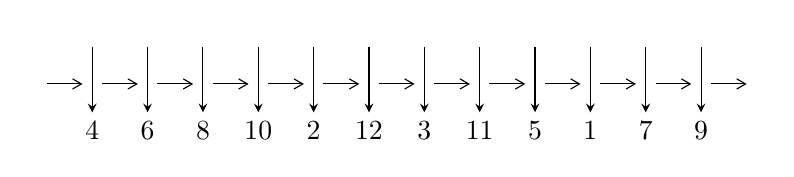
\begin{tikzpicture}[x=20pt, y=17pt]
	% nodes
	\node (C0) at (0, 0) {};
	\node (C1) at (1, 0) {};
	\node (C1U) at (1, +1) {};
	\node (C1D) at (1, -1) {4};

	\node (C2) at (2, 0) {};
	\node (C2U) at (2, +1) {};
	\node (C2D) at (2, -1) {6};

	\node (C3) at (3, 0) {};
	\node (C3U) at (3, +1) {};
	\node (C3D) at (3, -1) {8};

	\node (C4) at (4, 0) {};
	\node (C4U) at (4, +1) {};
	\node (C4D) at (4, -1) {10};

	\node (C5) at (5, 0) {};
	\node (C5U) at (5, +1) {};
	\node (C5D) at (5, -1) {2};

	\node (C6) at (6, 0) {};
	\node (C6U) at (6, +1) {};
	\node (C6D) at (6, -1) {12};

	\node (C7) at (7, 0) {};
	\node (C7U) at (7, +1) {};
	\node (C7D) at (7, -1) {3};

	\node (C8) at (8, 0) {};
	\node (C8U) at (8, +1) {};
	\node (C8D) at (8, -1) {11};

	\node (C9) at (9, 0) {};
	\node (C9U) at (9, +1) {};
	\node (C9D) at (9, -1) {5};

	\node (C10) at (10, 0) {};
	\node (C10U) at (10, +1) {};
	\node (C10D) at (10, -1) {1};

	\node (C11) at (11, 0) {};
	\node (C11U) at (11, +1) {};
	\node (C11D) at (11, -1) {7};

	\node (C12) at (12, 0) {};
	\node (C12U) at (12, +1) {};
	\node (C12D) at (12, -1) {9};
	\node (C13) at (13, 0) {};

	% arrows
	\draw[->,>={angle 60}]
	(C0) edge (C1) (C1) edge (C2) (C2) edge (C3) (C3) edge (C4) (C4) edge (C5) (C5) edge (C6) (C6) edge (C7) (C7) edge (C8) (C8) edge (C9) (C9) edge (C10) (C10) edge (C11) (C11) edge (C12) (C12) edge (C13) ;	\draw[->,>=stealth]
	(C1U) edge (C1D) (C2U) edge (C2D) (C3U) edge (C3D) (C4U) edge (C4D) (C5U) edge (C5D) (C6U) edge (C6D) (C7U) edge (C7D) (C8U) edge (C8D) (C9U) edge (C9D) (C10U) edge (C10D) (C11U) edge (C11D) (C12U) edge (C12D) ;
	\end{tikzpicture} \\
\hhline{~~} \\& 
\textbf{Solving Sequence} \\ \cline{2-2} 
 &
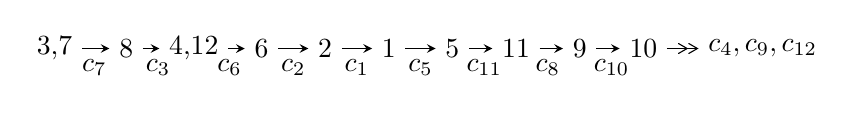
\begin{tikzpicture}[x=23pt, y=7pt]
	% node
	\node (A0) at (-1/8, 0) {3,7};
	\node (A1) at (1, 0) {8};
	\node (A2) at (33/16, 0) {4,12};
	\node (A3) at (25/8, 0) {6};
	\node (A4) at (33/8, 0) {2};
	\node (A5) at (41/8, 0) {1};
	\node (A6) at (49/8, 0) {5};
	\node (A7) at (57/8, 0) {11};
	\node (A8) at (65/8, 0) {9};
	\node (A9) at (73/8, 0) {10};
	\node (C1) at (1/2, -1) {$c_{7}$};
	\node (C2) at (3/2, -1) {$c_{3}$};
	\node (C3) at (21/8, -1) {$c_{6}$};
	\node (C4) at (29/8, -1) {$c_{2}$};
	\node (C5) at (37/8, -1) {$c_{1}$};
	\node (C6) at (45/8, -1) {$c_{5}$};
	\node (C7) at (53/8, -1) {$c_{11}$};
	\node (C8) at (61/8, -1) {$c_{8}$};
	\node (C9) at (69/8, -1) {$c_{10}$};
	\node (A10) at (11, 0) {$c_{4},c_{9},c_{12}$};

	% edge
	\draw[->,>=stealth]	
	(A0) edge (A1) (A1) edge (A2) (A2) edge (A3) (A3) edge (A4) (A4) edge (A5) (A5) edge (A6) (A6) edge (A7) (A7) edge (A8) (A8) edge (A9) ;
	\draw[->>,>={angle 60}]	
	(A9) edge (A10);
\end{tikzpicture} \\ 

\end{tabular} \\

\footnotetext{
The image of knot diagram is generated by the software ``\textbf{Draw programme}" developed by Andrew Bartholomew(\url{http://www.layer8.co.uk/maths/draw/index.htm\#Running-draw}), where we modified some parts for our purpose(\url{https://github.com/CATsTAILs/LinksPainter}).
}\phantom \\ \newline 
\centering \textbf{Ideals for irreducible components\footnotemark of $X_{\text{par}}$} 
 
\begin{align*}
I^u_{1}&=\langle 
8.52837\times10^{1076} u^{168}+9.95193\times10^{1076} u^{167}+\cdots+5.83099\times10^{1076} b-7.56901\times10^{1081},\\
\phantom{I^u_{1}}&\phantom{= \langle  }7.17815\times10^{1082} u^{168}+8.07968\times10^{1082} u^{167}+\cdots+2.21108\times10^{1082} a-6.04767\times10^{1087},\\
\phantom{I^u_{1}}&\phantom{= \langle  }u^{169}+2 u^{168}+\cdots-373810 u-75839\rangle \\
I^u_{2}&=\langle 
-6.31697\times10^{64} u^{45}-2.06195\times10^{65} u^{44}+\cdots+7.62817\times10^{64} b-3.63136\times10^{65},\\
\phantom{I^u_{2}}&\phantom{= \langle  }-1.17290\times10^{66} u^{45}-1.34273\times10^{66} u^{44}+\cdots+3.81409\times10^{65} a+1.51650\times10^{66},\;u^{46}+u^{45}+\cdots-4 u-1\rangle \\
\\
\end{align*}
\raggedright * 2 irreducible components of $\dim_{\mathbb{C}}=0$, with total 215 representations.\\
\footnotetext{All coefficients of polynomials are rational numbers. But the coefficients are sometimes approximated in decimal forms when there is not enough margin.}
\newpage
\renewcommand{\arraystretch}{1}
\centering \section*{I. $I^u_{1}= \langle 8.53\times10^{1076} u^{168}+9.95\times10^{1076} u^{167}+\cdots+5.83\times10^{1076} b-7.57\times10^{1081},\;7.18\times10^{1082} u^{168}+8.08\times10^{1082} u^{167}+\cdots+2.21\times10^{1082} a-6.05\times10^{1087},\;u^{169}+2 u^{168}+\cdots-373810 u-75839 \rangle$}
\flushleft \textbf{(i) Arc colorings}\\
\begin{tabular}{m{7pt} m{180pt} m{7pt} m{180pt} }
\flushright $a_{3}=$&$\begin{pmatrix}0\\u\end{pmatrix}$ \\
\flushright $a_{7}=$&$\begin{pmatrix}1\\0\end{pmatrix}$ \\
\flushright $a_{8}=$&$\begin{pmatrix}1\\u^2\end{pmatrix}$ \\
\flushright $a_{4}=$&$\begin{pmatrix}- u\\- u^3+u\end{pmatrix}$ \\
\flushright $a_{12}=$&$\begin{pmatrix}-3.24644 u^{168}-3.65417 u^{167}+\cdots+1.05369\times10^{6} u+273516.\\-1.46259 u^{168}-1.70673 u^{167}+\cdots+491774. u+129807.\end{pmatrix}$ \\
\flushright $a_{6}=$&$\begin{pmatrix}-1.43362 u^{168}-1.83638 u^{167}+\cdots+526370. u+144064.\\-0.217014 u^{168}-0.678800 u^{167}+\cdots+186090. u+61996.7\end{pmatrix}$ \\
\flushright $a_{2}=$&$\begin{pmatrix}-2.16396 u^{168}-2.54382 u^{167}+\cdots+731440. u+193639.\\0.821662 u^{168}+0.668477 u^{167}+\cdots-197557. u-43523.6\end{pmatrix}$ \\
\flushright $a_{1}=$&$\begin{pmatrix}-1.70674 u^{168}-2.18349 u^{167}+\cdots+624681. u+170586.\\0.971008 u^{168}+0.901172 u^{167}+\cdots-263253. u-62493.9\end{pmatrix}$ \\
\flushright $a_{5}=$&$\begin{pmatrix}-1.14675 u^{168}-1.51928 u^{167}+\cdots+432623. u+120017.\\-2.14197 u^{168}-2.47607 u^{167}+\cdots+714895. u+187876.\end{pmatrix}$ \\
\flushright $a_{11}=$&$\begin{pmatrix}-4.70903 u^{168}-5.36090 u^{167}+\cdots+1.54547\times10^{6} u+403323.\\-1.46259 u^{168}-1.70673 u^{167}+\cdots+491774. u+129807.\end{pmatrix}$ \\
\flushright $a_{9}=$&$\begin{pmatrix}0.225879 u^{168}+0.766581 u^{167}+\cdots-213899. u-72749.7\\0.107099 u^{168}+0.0596876 u^{167}+\cdots-17426.1 u-2380.89\end{pmatrix}$ \\
\flushright $a_{10}=$&$\begin{pmatrix}-2.78009 u^{168}-2.70356 u^{167}+\cdots+797029. u+193308.\\-0.108139 u^{168}-0.159883 u^{167}+\cdots+42772.8 u+11675.4\end{pmatrix}$\\&\end{tabular}
\flushleft \textbf{(ii) Obstruction class $= -1$}\\~\\
\flushleft \textbf{(iii) Cusp Shapes $= -5.62131 u^{168}-6.90171 u^{167}+\cdots+1.99401\times10^{6} u+538459.$}\\~\\
\newpage\renewcommand{\arraystretch}{1}
\flushleft \textbf{(iv) u-Polynomials at the component}\newline \\
\begin{tabular}{m{50pt}|m{274pt}}
Crossings & \hspace{64pt}u-Polynomials at each crossing \\
\hline $$\begin{aligned}c_{1}\end{aligned}$$&$\begin{aligned}
&u^{169}-10 u^{168}+\cdots-8577 u+415
\end{aligned}$\\
\hline $$\begin{aligned}c_{2},c_{5}\end{aligned}$$&$\begin{aligned}
&5(5 u^{169}-24 u^{168}+\cdots+3.48029\times10^{8} u+2.48668\times10^{7})
\end{aligned}$\\
\hline $$\begin{aligned}c_{3},c_{7}\end{aligned}$$&$\begin{aligned}
&u^{169}-2 u^{168}+\cdots-373810 u+75839
\end{aligned}$\\
\hline $$\begin{aligned}c_{4},c_{9}\end{aligned}$$&$\begin{aligned}
&u^{169}- u^{168}+\cdots-1899 u+373
\end{aligned}$\\
\hline $$\begin{aligned}c_{6},c_{11}\end{aligned}$$&$\begin{aligned}
&u^{169}+2 u^{168}+\cdots+184 u+193
\end{aligned}$\\
\hline $$\begin{aligned}c_{8}\end{aligned}$$&$\begin{aligned}
&5(5 u^{169}-83 u^{168}+\cdots-1136881 u+191311)
\end{aligned}$\\
\hline $$\begin{aligned}c_{10}\end{aligned}$$&$\begin{aligned}
&5(5 u^{169}-13 u^{168}+\cdots-845357 u+161671)
\end{aligned}$\\
\hline $$\begin{aligned}c_{12}\end{aligned}$$&$\begin{aligned}
&u^{169}+3 u^{168}+\cdots-19434 u+2711
\end{aligned}$\\
\hline
\end{tabular}\\~\\
\newpage\renewcommand{\arraystretch}{1}
\flushleft \textbf{(v) Riley Polynomials at the component}\newline \\
\begin{tabular}{m{50pt}|m{274pt}}
Crossings & \hspace{64pt}Riley Polynomials at each crossing \\
\hline $$\begin{aligned}c_{1}\end{aligned}$$&$\begin{aligned}
&y^{169}-14 y^{168}+\cdots-98510671 y-172225
\end{aligned}$\\
\hline $$\begin{aligned}c_{2},c_{5}\end{aligned}$$&$\begin{aligned}
&25\\
&\cdot(25 y^{169}-3896 y^{168}+\cdots+10579956017594239 y-618357294637681)
\end{aligned}$\\
\hline $$\begin{aligned}c_{3},c_{7}\end{aligned}$$&$\begin{aligned}
&y^{169}-100 y^{168}+\cdots+233540843658 y-5751553921
\end{aligned}$\\
\hline $$\begin{aligned}c_{4},c_{9}\end{aligned}$$&$\begin{aligned}
&y^{169}+95 y^{168}+\cdots-4640829 y-139129
\end{aligned}$\\
\hline $$\begin{aligned}c_{6},c_{11}\end{aligned}$$&$\begin{aligned}
&y^{169}+80 y^{168}+\cdots-1198642 y-37249
\end{aligned}$\\
\hline $$\begin{aligned}c_{8}\end{aligned}$$&$\begin{aligned}
&25(25 y^{169}+1011 y^{168}+\cdots-2.93882\times10^{12} y-3.65999\times10^{10})
\end{aligned}$\\
\hline $$\begin{aligned}c_{10}\end{aligned}$$&$\begin{aligned}
&25(25 y^{169}+1711 y^{168}+\cdots-3.11859\times10^{11} y-2.61375\times10^{10})
\end{aligned}$\\
\hline $$\begin{aligned}c_{12}\end{aligned}$$&$\begin{aligned}
&y^{169}+35 y^{168}+\cdots+1287952826 y-7349521
\end{aligned}$\\
\hline
\end{tabular}\\~\\
\newpage\flushleft \textbf{(vi) Complex Volumes and Cusp Shapes}
$$\begin{array}{c|c|c}  
\text{Solutions to }I^u_{1}& \I (\text{vol} + \sqrt{-1}CS) & \text{Cusp shape}\\
 \hline 
\begin{aligned}
u &= \phantom{-}0.784708 + 0.613924 I \\
a &= -0.643559 + 0.808589 I \\
b &= \phantom{-}0.37279 - 1.37564 I\end{aligned}
 & \phantom{-}5.44300 - 3.46467 I & \phantom{-0.000000 } 0 \\ \hline\begin{aligned}
u &= \phantom{-}0.784708 - 0.613924 I \\
a &= -0.643559 - 0.808589 I \\
b &= \phantom{-}0.37279 + 1.37564 I\end{aligned}
 & \phantom{-}5.44300 + 3.46467 I & \phantom{-0.000000 } 0 \\ \hline\begin{aligned}
u &= \phantom{-}0.920244 + 0.377047 I \\
a &= \phantom{-}1.60054 + 0.02840 I \\
b &= -0.097204 + 0.531932 I\end{aligned}
 & -1.33676 - 1.43995 I & \phantom{-0.000000 } 0 \\ \hline\begin{aligned}
u &= \phantom{-}0.920244 - 0.377047 I \\
a &= \phantom{-}1.60054 - 0.02840 I \\
b &= -0.097204 - 0.531932 I\end{aligned}
 & -1.33676 + 1.43995 I & \phantom{-0.000000 } 0 \\ \hline\begin{aligned}
u &= \phantom{-}0.915176 + 0.374176 I \\
a &= -0.881069 + 0.421708 I \\
b &= -0.665475 + 0.344780 I\end{aligned}
 & -1.61762 - 3.68106 I & \phantom{-0.000000 } 0 \\ \hline\begin{aligned}
u &= \phantom{-}0.915176 - 0.374176 I \\
a &= -0.881069 - 0.421708 I \\
b &= -0.665475 - 0.344780 I\end{aligned}
 & -1.61762 + 3.68106 I & \phantom{-0.000000 } 0 \\ \hline\begin{aligned}
u &= -0.911314 + 0.371165 I \\
a &= -0.962164 - 0.086599 I \\
b &= -0.296551 + 1.206580 I\end{aligned}
 & \phantom{-}4.32077 - 5.45772 I & \phantom{-0.000000 } 0 \\ \hline\begin{aligned}
u &= -0.911314 - 0.371165 I \\
a &= -0.962164 + 0.086599 I \\
b &= -0.296551 - 1.206580 I\end{aligned}
 & \phantom{-}4.32077 + 5.45772 I & \phantom{-0.000000 } 0 \\ \hline\begin{aligned}
u &= \phantom{-}0.830216 + 0.518276 I \\
a &= -1.09985 + 1.20733 I \\
b &= -0.662634 - 1.196350 I\end{aligned}
 & \phantom{-}5.28936 - 1.07756 I & \phantom{-0.000000 } 0 \\ \hline\begin{aligned}
u &= \phantom{-}0.830216 - 0.518276 I \\
a &= -1.09985 - 1.20733 I \\
b &= -0.662634 + 1.196350 I\end{aligned}
 & \phantom{-}5.28936 + 1.07756 I & \phantom{-0.000000 } 0\\
 \hline 
 \end{array}$$\newpage$$\begin{array}{c|c|c}  
\text{Solutions to }I^u_{1}& \I (\text{vol} + \sqrt{-1}CS) & \text{Cusp shape}\\
 \hline 
\begin{aligned}
u &= \phantom{-}0.267064 + 0.928594 I \\
a &= \phantom{-}0.78004 - 1.30401 I \\
b &= -0.476011 + 0.994886 I\end{aligned}
 & -1.29765 + 2.45359 I & \phantom{-0.000000 } 0 \\ \hline\begin{aligned}
u &= \phantom{-}0.267064 - 0.928594 I \\
a &= \phantom{-}0.78004 + 1.30401 I \\
b &= -0.476011 - 0.994886 I\end{aligned}
 & -1.29765 - 2.45359 I & \phantom{-0.000000 } 0 \\ \hline\begin{aligned}
u &= \phantom{-}0.865667 + 0.411875 I \\
a &= \phantom{-}1.023270 - 0.122811 I \\
b &= \phantom{-}0.332039 + 0.960787 I\end{aligned}
 & \phantom{-}0.593196 + 0.743247 I & \phantom{-0.000000 } 0 \\ \hline\begin{aligned}
u &= \phantom{-}0.865667 - 0.411875 I \\
a &= \phantom{-}1.023270 + 0.122811 I \\
b &= \phantom{-}0.332039 - 0.960787 I\end{aligned}
 & \phantom{-}0.593196 - 0.743247 I & \phantom{-0.000000 } 0 \\ \hline\begin{aligned}
u &= \phantom{-}0.268756 + 1.009500 I \\
a &= -0.41582 + 1.58361 I \\
b &= \phantom{-}0.429135 - 0.496965 I\end{aligned}
 & -2.14568 - 2.88218 I & \phantom{-0.000000 } 0 \\ \hline\begin{aligned}
u &= \phantom{-}0.268756 - 1.009500 I \\
a &= -0.41582 - 1.58361 I \\
b &= \phantom{-}0.429135 + 0.496965 I\end{aligned}
 & -2.14568 + 2.88218 I & \phantom{-0.000000 } 0 \\ \hline\begin{aligned}
u &= \phantom{-}0.260589 + 0.911776 I \\
a &= -0.51091 - 1.51427 I \\
b &= -0.086537 + 1.184460 I\end{aligned}
 & \phantom{-}7.21873 - 2.31414 I & \phantom{-0.000000 } 0 \\ \hline\begin{aligned}
u &= \phantom{-}0.260589 - 0.911776 I \\
a &= -0.51091 + 1.51427 I \\
b &= -0.086537 - 1.184460 I\end{aligned}
 & \phantom{-}7.21873 + 2.31414 I & \phantom{-0.000000 } 0 \\ \hline\begin{aligned}
u &= -0.928179 + 0.185085 I \\
a &= -1.31562 - 1.02496 I \\
b &= -0.496072 + 0.506207 I\end{aligned}
 & -3.28092 + 0.65320 I & \phantom{-0.000000 } 0 \\ \hline\begin{aligned}
u &= -0.928179 - 0.185085 I \\
a &= -1.31562 + 1.02496 I \\
b &= -0.496072 - 0.506207 I\end{aligned}
 & -3.28092 - 0.65320 I & \phantom{-0.000000 } 0\\
 \hline 
 \end{array}$$\newpage$$\begin{array}{c|c|c}  
\text{Solutions to }I^u_{1}& \I (\text{vol} + \sqrt{-1}CS) & \text{Cusp shape}\\
 \hline 
\begin{aligned}
u &= -0.722890 + 0.603420 I \\
a &= -0.332399 + 0.483389 I \\
b &= -0.243722 - 0.338431 I\end{aligned}
 & \phantom{-}2.71954 + 3.65187 I & \phantom{-0.000000 } 0 \\ \hline\begin{aligned}
u &= -0.722890 - 0.603420 I \\
a &= -0.332399 - 0.483389 I \\
b &= -0.243722 + 0.338431 I\end{aligned}
 & \phantom{-}2.71954 - 3.65187 I & \phantom{-0.000000 } 0 \\ \hline\begin{aligned}
u &= -1.019350 + 0.308406 I \\
a &= -1.96904 + 0.11380 I \\
b &= \phantom{-}0.078671 + 0.716499 I\end{aligned}
 & -1.352700 - 0.345590 I & \phantom{-0.000000 } 0 \\ \hline\begin{aligned}
u &= -1.019350 - 0.308406 I \\
a &= -1.96904 - 0.11380 I \\
b &= \phantom{-}0.078671 - 0.716499 I\end{aligned}
 & -1.352700 + 0.345590 I & \phantom{-0.000000 } 0 \\ \hline\begin{aligned}
u &= \phantom{-}0.933309 + 0.043329 I \\
a &= \phantom{-}2.70551 - 5.68153 I \\
b &= \phantom{-}0.118826 + 1.029770 I\end{aligned}
 & \phantom{-}0.182079 - 0.083509 I & \phantom{-0.000000 } 0 \\ \hline\begin{aligned}
u &= \phantom{-}0.933309 - 0.043329 I \\
a &= \phantom{-}2.70551 + 5.68153 I \\
b &= \phantom{-}0.118826 - 1.029770 I\end{aligned}
 & \phantom{-}0.182079 + 0.083509 I & \phantom{-0.000000 } 0 \\ \hline\begin{aligned}
u &= \phantom{-}0.741521 + 0.766665 I \\
a &= -0.80312 + 1.48660 I \\
b &= -0.791649 - 0.938174 I\end{aligned}
 & \phantom{-}2.65700 - 8.59855 I & \phantom{-0.000000 } 0 \\ \hline\begin{aligned}
u &= \phantom{-}0.741521 - 0.766665 I \\
a &= -0.80312 - 1.48660 I \\
b &= -0.791649 + 0.938174 I\end{aligned}
 & \phantom{-}2.65700 + 8.59855 I & \phantom{-0.000000 } 0 \\ \hline\begin{aligned}
u &= \phantom{-}1.084770 + 0.075835 I \\
a &= \phantom{-}0.676752 - 0.593636 I \\
b &= \phantom{-}0.635917 + 0.164215 I\end{aligned}
 & -1.44974 + 2.38111 I & \phantom{-0.000000 } 0 \\ \hline\begin{aligned}
u &= \phantom{-}1.084770 - 0.075835 I \\
a &= \phantom{-}0.676752 + 0.593636 I \\
b &= \phantom{-}0.635917 - 0.164215 I\end{aligned}
 & -1.44974 - 2.38111 I & \phantom{-0.000000 } 0\\
 \hline 
 \end{array}$$\newpage$$\begin{array}{c|c|c}  
\text{Solutions to }I^u_{1}& \I (\text{vol} + \sqrt{-1}CS) & \text{Cusp shape}\\
 \hline 
\begin{aligned}
u &= -0.967024 + 0.504518 I \\
a &= \phantom{-}0.636371 + 0.801048 I \\
b &= \phantom{-}0.821785 - 0.053503 I\end{aligned}
 & \phantom{-}1.22501 + 8.45758 I & \phantom{-0.000000 } 0 \\ \hline\begin{aligned}
u &= -0.967024 - 0.504518 I \\
a &= \phantom{-}0.636371 - 0.801048 I \\
b &= \phantom{-}0.821785 + 0.053503 I\end{aligned}
 & \phantom{-}1.22501 - 8.45758 I & \phantom{-0.000000 } 0 \\ \hline\begin{aligned}
u &= -1.089940 + 0.203333 I \\
a &= \phantom{-}1.71443 + 0.58971 I \\
b &= \phantom{-}0.354122 - 1.083020 I\end{aligned}
 & \phantom{-}1.79023 + 0.79732 I & \phantom{-0.000000 } 0 \\ \hline\begin{aligned}
u &= -1.089940 - 0.203333 I \\
a &= \phantom{-}1.71443 - 0.58971 I \\
b &= \phantom{-}0.354122 + 1.083020 I\end{aligned}
 & \phantom{-}1.79023 - 0.79732 I & \phantom{-0.000000 } 0 \\ \hline\begin{aligned}
u &= -0.665123 + 0.890537 I \\
a &= \phantom{-}0.284939 + 0.666179 I \\
b &= -0.540626 - 0.822974 I\end{aligned}
 & \phantom{-}2.50535 + 3.30834 I & \phantom{-0.000000 } 0 \\ \hline\begin{aligned}
u &= -0.665123 - 0.890537 I \\
a &= \phantom{-}0.284939 - 0.666179 I \\
b &= -0.540626 + 0.822974 I\end{aligned}
 & \phantom{-}2.50535 - 3.30834 I & \phantom{-0.000000 } 0 \\ \hline\begin{aligned}
u &= -0.873663 + 0.146201 I \\
a &= -0.083774 - 1.203770 I \\
b &= \phantom{-}0.01017 + 1.81847 I\end{aligned}
 & \phantom{-}4.92828 + 7.63290 I & \phantom{-0.000000 } 0 \\ \hline\begin{aligned}
u &= -0.873663 - 0.146201 I \\
a &= -0.083774 + 1.203770 I \\
b &= \phantom{-}0.01017 - 1.81847 I\end{aligned}
 & \phantom{-}4.92828 - 7.63290 I & \phantom{-0.000000 } 0 \\ \hline\begin{aligned}
u &= -0.844903 + 0.254381 I \\
a &= \phantom{-}0.398836 - 1.045490 I \\
b &= \phantom{-}0.33666 + 1.42613 I\end{aligned}
 & \phantom{-}4.42997 - 1.35438 I & \phantom{-0.000000 } 0 \\ \hline\begin{aligned}
u &= -0.844903 - 0.254381 I \\
a &= \phantom{-}0.398836 + 1.045490 I \\
b &= \phantom{-}0.33666 - 1.42613 I\end{aligned}
 & \phantom{-}4.42997 + 1.35438 I & \phantom{-0.000000 } 0\\
 \hline 
 \end{array}$$\newpage$$\begin{array}{c|c|c}  
\text{Solutions to }I^u_{1}& \I (\text{vol} + \sqrt{-1}CS) & \text{Cusp shape}\\
 \hline 
\begin{aligned}
u &= -0.807222 + 0.336582 I \\
a &= -1.070950 - 0.039143 I \\
b &= -0.651460 + 0.967818 I\end{aligned}
 & \phantom{-}4.35010 + 4.01737 I & \phantom{-0.000000 } 0 \\ \hline\begin{aligned}
u &= -0.807222 - 0.336582 I \\
a &= -1.070950 + 0.039143 I \\
b &= -0.651460 - 0.967818 I\end{aligned}
 & \phantom{-}4.35010 - 4.01737 I & \phantom{-0.000000 } 0 \\ \hline\begin{aligned}
u &= -0.208446 + 0.846554 I \\
a &= -0.68762 - 1.46932 I \\
b &= \phantom{-}0.543847 + 1.119410 I\end{aligned}
 & \phantom{-}0.17317 - 6.34643 I & \phantom{-0.000000 } 0 \\ \hline\begin{aligned}
u &= -0.208446 - 0.846554 I \\
a &= -0.68762 + 1.46932 I \\
b &= \phantom{-}0.543847 - 1.119410 I\end{aligned}
 & \phantom{-}0.17317 + 6.34643 I & \phantom{-0.000000 } 0 \\ \hline\begin{aligned}
u &= -0.862498 + 0.731446 I \\
a &= -0.31807 - 1.82238 I \\
b &= -0.510474 + 0.892164 I\end{aligned}
 & -3.31588 + 2.03557 I & \phantom{-0.000000 } 0 \\ \hline\begin{aligned}
u &= -0.862498 - 0.731446 I \\
a &= -0.31807 + 1.82238 I \\
b &= -0.510474 - 0.892164 I\end{aligned}
 & -3.31588 - 2.03557 I & \phantom{-0.000000 } 0 \\ \hline\begin{aligned}
u &= -0.528278 + 0.683581 I \\
a &= \phantom{-}0.459538 + 1.239740 I \\
b &= -0.094965 - 1.184460 I\end{aligned}
 & \phantom{-}3.30392 + 1.21744 I & \phantom{-0.000000 } 0 \\ \hline\begin{aligned}
u &= -0.528278 - 0.683581 I \\
a &= \phantom{-}0.459538 - 1.239740 I \\
b &= -0.094965 + 1.184460 I\end{aligned}
 & \phantom{-}3.30392 - 1.21744 I & \phantom{-0.000000 } 0 \\ \hline\begin{aligned}
u &= -0.850837 + 0.148530 I \\
a &= -1.44220 - 1.52687 I \\
b &= -0.635119 + 0.854070 I\end{aligned}
 & -3.31379 + 1.12851 I & \phantom{-0.000000 } 0 \\ \hline\begin{aligned}
u &= -0.850837 - 0.148530 I \\
a &= -1.44220 + 1.52687 I \\
b &= -0.635119 - 0.854070 I\end{aligned}
 & -3.31379 - 1.12851 I & \phantom{-0.000000 } 0\\
 \hline 
 \end{array}$$\newpage$$\begin{array}{c|c|c}  
\text{Solutions to }I^u_{1}& \I (\text{vol} + \sqrt{-1}CS) & \text{Cusp shape}\\
 \hline 
\begin{aligned}
u &= \phantom{-}1.113610 + 0.236527 I \\
a &= -0.0081692 - 0.1312360 I \\
b &= -1.50389 + 0.58738 I\end{aligned}
 & -4.64578 + 0.86236 I & \phantom{-0.000000 } 0 \\ \hline\begin{aligned}
u &= \phantom{-}1.113610 - 0.236527 I \\
a &= -0.0081692 + 0.1312360 I \\
b &= -1.50389 - 0.58738 I\end{aligned}
 & -4.64578 - 0.86236 I & \phantom{-0.000000 } 0 \\ \hline\begin{aligned}
u &= \phantom{-}0.231656 + 0.829785 I \\
a &= -0.05951 - 1.61145 I \\
b &= -0.299929 + 1.307960 I\end{aligned}
 & \phantom{-}7.72074 + 8.11198 I & \phantom{-0.000000 } 0 \\ \hline\begin{aligned}
u &= \phantom{-}0.231656 - 0.829785 I \\
a &= -0.05951 + 1.61145 I \\
b &= -0.299929 - 1.307960 I\end{aligned}
 & \phantom{-}7.72074 - 8.11198 I & \phantom{-0.000000 } 0 \\ \hline\begin{aligned}
u &= \phantom{-}0.853699 + 0.104903 I \\
a &= \phantom{-}0.95430 - 1.54712 I \\
b &= \phantom{-}0.68482 + 1.28338 I\end{aligned}
 & -1.92543 - 4.84905 I & \phantom{-0.000000 } 0 \\ \hline\begin{aligned}
u &= \phantom{-}0.853699 - 0.104903 I \\
a &= \phantom{-}0.95430 + 1.54712 I \\
b &= \phantom{-}0.68482 - 1.28338 I\end{aligned}
 & -1.92543 + 4.84905 I & \phantom{-0.000000 } 0 \\ \hline\begin{aligned}
u &= -0.847346 + 0.133559 I \\
a &= \phantom{-}1.63878 - 0.39556 I \\
b &= \phantom{-}0.276780 + 0.779594 I\end{aligned}
 & \phantom{-}3.11053 - 0.19176 I & \phantom{-0.000000 } 0 \\ \hline\begin{aligned}
u &= -0.847346 - 0.133559 I \\
a &= \phantom{-}1.63878 + 0.39556 I \\
b &= \phantom{-}0.276780 - 0.779594 I\end{aligned}
 & \phantom{-}3.11053 + 0.19176 I & \phantom{-0.000000 } 0 \\ \hline\begin{aligned}
u &= -0.022376 + 0.855453 I \\
a &= \phantom{-}0.90417 - 1.31054 I \\
b &= -0.429783 + 1.209360 I\end{aligned}
 & \phantom{-}1.59238 + 4.23637 I & \phantom{-0.000000 } 0 \\ \hline\begin{aligned}
u &= -0.022376 - 0.855453 I \\
a &= \phantom{-}0.90417 + 1.31054 I \\
b &= -0.429783 - 1.209360 I\end{aligned}
 & \phantom{-}1.59238 - 4.23637 I & \phantom{-0.000000 } 0\\
 \hline 
 \end{array}$$\newpage$$\begin{array}{c|c|c}  
\text{Solutions to }I^u_{1}& \I (\text{vol} + \sqrt{-1}CS) & \text{Cusp shape}\\
 \hline 
\begin{aligned}
u &= \phantom{-}0.839044 + 0.145941 I \\
a &= -0.08746 - 1.42549 I \\
b &= \phantom{-}0.00710 + 1.56514 I\end{aligned}
 & \phantom{-}1.27540 - 3.22857 I & \phantom{-0.000000 } 0 \\ \hline\begin{aligned}
u &= \phantom{-}0.839044 - 0.145941 I \\
a &= -0.08746 + 1.42549 I \\
b &= \phantom{-}0.00710 - 1.56514 I\end{aligned}
 & \phantom{-}1.27540 + 3.22857 I & \phantom{-0.000000 } 0 \\ \hline\begin{aligned}
u &= -0.277337 + 0.804585 I \\
a &= \phantom{-}0.164515 - 1.317430 I \\
b &= \phantom{-}0.274774 + 1.190640 I\end{aligned}
 & \phantom{-}3.45365 - 3.41412 I & \phantom{-0.000000 } 0 \\ \hline\begin{aligned}
u &= -0.277337 - 0.804585 I \\
a &= \phantom{-}0.164515 + 1.317430 I \\
b &= \phantom{-}0.274774 - 1.190640 I\end{aligned}
 & \phantom{-}3.45365 + 3.41412 I & \phantom{-0.000000 } 0 \\ \hline\begin{aligned}
u &= \phantom{-}1.120720 + 0.336689 I \\
a &= \phantom{-}0.003701 + 0.171555 I \\
b &= -1.271420 + 0.543908 I\end{aligned}
 & -5.42015 - 4.37598 I & \phantom{-0.000000 } 0 \\ \hline\begin{aligned}
u &= \phantom{-}1.120720 - 0.336689 I \\
a &= \phantom{-}0.003701 - 0.171555 I \\
b &= -1.271420 - 0.543908 I\end{aligned}
 & -5.42015 + 4.37598 I & \phantom{-0.000000 } 0 \\ \hline\begin{aligned}
u &= -1.011570 + 0.588491 I \\
a &= \phantom{-}0.880891 + 1.061040 I \\
b &= \phantom{-}0.495034 - 1.040080 I\end{aligned}
 & \phantom{-}1.87354 + 3.75211 I & \phantom{-0.000000 } 0 \\ \hline\begin{aligned}
u &= -1.011570 - 0.588491 I \\
a &= \phantom{-}0.880891 - 1.061040 I \\
b &= \phantom{-}0.495034 + 1.040080 I\end{aligned}
 & \phantom{-}1.87354 - 3.75211 I & \phantom{-0.000000 } 0 \\ \hline\begin{aligned}
u &= -1.187150 + 0.225281 I \\
a &= -0.084077 - 0.115206 I \\
b &= \phantom{-}1.387830 + 0.195997 I\end{aligned}
 & -6.25555 + 1.65412 I & \phantom{-0.000000 } 0 \\ \hline\begin{aligned}
u &= -1.187150 - 0.225281 I \\
a &= -0.084077 + 0.115206 I \\
b &= \phantom{-}1.387830 - 0.195997 I\end{aligned}
 & -6.25555 - 1.65412 I & \phantom{-0.000000 } 0\\
 \hline 
 \end{array}$$\newpage$$\begin{array}{c|c|c}  
\text{Solutions to }I^u_{1}& \I (\text{vol} + \sqrt{-1}CS) & \text{Cusp shape}\\
 \hline 
\begin{aligned}
u &= -0.204359 + 0.762631 I \\
a &= \phantom{-}0.65317 + 1.81794 I \\
b &= -0.544913 - 0.241877 I\end{aligned}
 & \phantom{-}0.55143 + 9.06486 I & \phantom{-0.000000 } 0 \\ \hline\begin{aligned}
u &= -0.204359 - 0.762631 I \\
a &= \phantom{-}0.65317 - 1.81794 I \\
b &= -0.544913 + 0.241877 I\end{aligned}
 & \phantom{-}0.55143 - 9.06486 I & \phantom{-0.000000 } 0 \\ \hline\begin{aligned}
u &= -0.049278 + 0.780179 I \\
a &= -0.780221 - 1.046110 I \\
b &= \phantom{-}0.472046 + 1.129250 I\end{aligned}
 & \phantom{-}1.32461 - 2.32482 I & \phantom{-0.000000 } 0 \\ \hline\begin{aligned}
u &= -0.049278 - 0.780179 I \\
a &= -0.780221 + 1.046110 I \\
b &= \phantom{-}0.472046 - 1.129250 I\end{aligned}
 & \phantom{-}1.32461 + 2.32482 I & \phantom{-0.000000 } 0 \\ \hline\begin{aligned}
u &= -1.175890 + 0.326749 I \\
a &= -0.180592 + 0.035328 I \\
b &= \phantom{-}1.176990 + 0.557577 I\end{aligned}
 & -6.59949 + 1.11760 I & \phantom{-0.000000 } 0 \\ \hline\begin{aligned}
u &= -1.175890 - 0.326749 I \\
a &= -0.180592 - 0.035328 I \\
b &= \phantom{-}1.176990 - 0.557577 I\end{aligned}
 & -6.59949 - 1.11760 I & \phantom{-0.000000 } 0 \\ \hline\begin{aligned}
u &= -0.966156 + 0.783023 I \\
a &= \phantom{-}0.68210 + 1.26288 I \\
b &= \phantom{-}0.724741 - 0.867423 I\end{aligned}
 & \phantom{-}1.63076 + 2.82752 I & \phantom{-0.000000 } 0 \\ \hline\begin{aligned}
u &= -0.966156 - 0.783023 I \\
a &= \phantom{-}0.68210 - 1.26288 I \\
b &= \phantom{-}0.724741 + 0.867423 I\end{aligned}
 & \phantom{-}1.63076 - 2.82752 I & \phantom{-0.000000 } 0 \\ \hline\begin{aligned}
u &= \phantom{-}1.229220 + 0.244301 I \\
a &= -0.801288 + 0.253368 I \\
b &= -0.499729 - 1.033100 I\end{aligned}
 & -1.69948 - 3.50347 I & \phantom{-0.000000 } 0 \\ \hline\begin{aligned}
u &= \phantom{-}1.229220 - 0.244301 I \\
a &= -0.801288 - 0.253368 I \\
b &= -0.499729 + 1.033100 I\end{aligned}
 & -1.69948 + 3.50347 I & \phantom{-0.000000 } 0\\
 \hline 
 \end{array}$$\newpage$$\begin{array}{c|c|c}  
\text{Solutions to }I^u_{1}& \I (\text{vol} + \sqrt{-1}CS) & \text{Cusp shape}\\
 \hline 
\begin{aligned}
u &= -1.234680 + 0.277061 I \\
a &= \phantom{-}0.99756 + 1.58457 I \\
b &= \phantom{-}0.489008 - 1.112440 I\end{aligned}
 & -2.72337 + 10.53720 I & \phantom{-0.000000 } 0 \\ \hline\begin{aligned}
u &= -1.234680 - 0.277061 I \\
a &= \phantom{-}0.99756 - 1.58457 I \\
b &= \phantom{-}0.489008 + 1.112440 I\end{aligned}
 & -2.72337 - 10.53720 I & \phantom{-0.000000 } 0 \\ \hline\begin{aligned}
u &= \phantom{-}0.914174 + 0.878055 I \\
a &= -0.318771 + 0.651893 I \\
b &= \phantom{-}0.630963 - 1.009040 I\end{aligned}
 & \phantom{-}2.23701 + 2.52987 I & \phantom{-0.000000 } 0 \\ \hline\begin{aligned}
u &= \phantom{-}0.914174 - 0.878055 I \\
a &= -0.318771 - 0.651893 I \\
b &= \phantom{-}0.630963 + 1.009040 I\end{aligned}
 & \phantom{-}2.23701 - 2.52987 I & \phantom{-0.000000 } 0 \\ \hline\begin{aligned}
u &= \phantom{-}0.273246 + 1.238690 I \\
a &= \phantom{-}0.026142 + 1.339540 I \\
b &= -0.100077 - 1.138070 I\end{aligned}
 & \phantom{-}7.55549 - 1.54678 I & \phantom{-0.000000 } 0 \\ \hline\begin{aligned}
u &= \phantom{-}0.273246 - 1.238690 I \\
a &= \phantom{-}0.026142 - 1.339540 I \\
b &= -0.100077 + 1.138070 I\end{aligned}
 & \phantom{-}7.55549 + 1.54678 I & \phantom{-0.000000 } 0 \\ \hline\begin{aligned}
u &= -1.243950 + 0.288511 I \\
a &= -0.173414 - 0.135763 I \\
b &= \phantom{-}0.984332 + 0.308673 I\end{aligned}
 & -6.34008 + 1.34512 I & \phantom{-0.000000 } 0 \\ \hline\begin{aligned}
u &= -1.243950 - 0.288511 I \\
a &= -0.173414 + 0.135763 I \\
b &= \phantom{-}0.984332 - 0.308673 I\end{aligned}
 & -6.34008 - 1.34512 I & \phantom{-0.000000 } 0 \\ \hline\begin{aligned}
u &= \phantom{-}1.275850 + 0.167588 I \\
a &= -0.043975 - 0.157354 I \\
b &= -0.920866 - 0.483509 I\end{aligned}
 & -4.24168 - 4.68064 I & \phantom{-0.000000 } 0 \\ \hline\begin{aligned}
u &= \phantom{-}1.275850 - 0.167588 I \\
a &= -0.043975 + 0.157354 I \\
b &= -0.920866 + 0.483509 I\end{aligned}
 & -4.24168 + 4.68064 I & \phantom{-0.000000 } 0\\
 \hline 
 \end{array}$$\newpage$$\begin{array}{c|c|c}  
\text{Solutions to }I^u_{1}& \I (\text{vol} + \sqrt{-1}CS) & \text{Cusp shape}\\
 \hline 
\begin{aligned}
u &= \phantom{-}0.710178 + 0.032326 I \\
a &= \phantom{-}1.49756 + 0.26139 I \\
b &= \phantom{-}1.316290 + 0.027298 I\end{aligned}
 & -2.78206 - 2.35655 I & \phantom{-0.000000 } 0 \\ \hline\begin{aligned}
u &= \phantom{-}0.710178 - 0.032326 I \\
a &= \phantom{-}1.49756 - 0.26139 I \\
b &= \phantom{-}1.316290 - 0.027298 I\end{aligned}
 & -2.78206 + 2.35655 I & \phantom{-0.000000 } 0 \\ \hline\begin{aligned}
u &= -0.706628 + 0.038033 I \\
a &= -1.88252 - 0.60845 I \\
b &= -1.135580 + 0.244864 I\end{aligned}
 & -3.88353 + 0.65865 I & \phantom{-0.000000 } 0 \\ \hline\begin{aligned}
u &= -0.706628 - 0.038033 I \\
a &= -1.88252 + 0.60845 I \\
b &= -1.135580 - 0.244864 I\end{aligned}
 & -3.88353 - 0.65865 I & \phantom{-0.000000 } 0 \\ \hline\begin{aligned}
u &= \phantom{-}0.419587 + 0.568542 I \\
a &= \phantom{-}1.37429 - 1.11986 I \\
b &= -0.525739 + 0.566558 I\end{aligned}
 & -2.50872 + 1.64985 I & \phantom{-0.000000 } 0 \\ \hline\begin{aligned}
u &= \phantom{-}0.419587 - 0.568542 I \\
a &= \phantom{-}1.37429 + 1.11986 I \\
b &= -0.525739 - 0.566558 I\end{aligned}
 & -2.50872 - 1.64985 I & \phantom{-0.000000 } 0 \\ \hline\begin{aligned}
u &= -0.336968 + 0.584671 I \\
a &= \phantom{-}0.257670 - 0.354689 I \\
b &= -0.791991 - 0.225991 I\end{aligned}
 & \phantom{-}2.93185 - 4.25246 I & \phantom{-0.000000 } 0 \\ \hline\begin{aligned}
u &= -0.336968 - 0.584671 I \\
a &= \phantom{-}0.257670 + 0.354689 I \\
b &= -0.791991 + 0.225991 I\end{aligned}
 & \phantom{-}2.93185 + 4.25246 I & \phantom{-0.000000 } 0 \\ \hline\begin{aligned}
u &= \phantom{-}1.229950 + 0.505940 I \\
a &= \phantom{-}1.21373 - 0.79773 I \\
b &= \phantom{-}0.505515 + 1.190320 I\end{aligned}
 & \phantom{-}4.59681 - 13.07660 I & \phantom{-0.000000 } 0 \\ \hline\begin{aligned}
u &= \phantom{-}1.229950 - 0.505940 I \\
a &= \phantom{-}1.21373 + 0.79773 I \\
b &= \phantom{-}0.505515 - 1.190320 I\end{aligned}
 & \phantom{-}4.59681 + 13.07660 I & \phantom{-0.000000 } 0\\
 \hline 
 \end{array}$$\newpage$$\begin{array}{c|c|c}  
\text{Solutions to }I^u_{1}& \I (\text{vol} + \sqrt{-1}CS) & \text{Cusp shape}\\
 \hline 
\begin{aligned}
u &= \phantom{-}1.254070 + 0.452267 I \\
a &= -0.0717085 - 0.0096982 I \\
b &= \phantom{-}1.275460 - 0.413555 I\end{aligned}
 & -3.43263 - 13.45390 I & \phantom{-0.000000 } 0 \\ \hline\begin{aligned}
u &= \phantom{-}1.254070 - 0.452267 I \\
a &= -0.0717085 + 0.0096982 I \\
b &= \phantom{-}1.275460 + 0.413555 I\end{aligned}
 & -3.43263 + 13.45390 I & \phantom{-0.000000 } 0 \\ \hline\begin{aligned}
u &= -1.219820 + 0.547229 I \\
a &= -0.84466 - 1.25709 I \\
b &= -0.75383 + 1.27190 I\end{aligned}
 & -2.88770 + 11.52210 I & \phantom{-0.000000 } 0 \\ \hline\begin{aligned}
u &= -1.219820 - 0.547229 I \\
a &= -0.84466 + 1.25709 I \\
b &= -0.75383 - 1.27190 I\end{aligned}
 & -2.88770 - 11.52210 I & \phantom{-0.000000 } 0 \\ \hline\begin{aligned}
u &= \phantom{-}1.142900 + 0.704290 I \\
a &= \phantom{-}0.44210 - 1.49246 I \\
b &= \phantom{-}0.625808 + 1.112300 I\end{aligned}
 & -4.03602 - 6.95926 I & \phantom{-0.000000 } 0 \\ \hline\begin{aligned}
u &= \phantom{-}1.142900 - 0.704290 I \\
a &= \phantom{-}0.44210 + 1.49246 I \\
b &= \phantom{-}0.625808 - 1.112300 I\end{aligned}
 & -4.03602 + 6.95926 I & \phantom{-0.000000 } 0 \\ \hline\begin{aligned}
u &= -1.238850 + 0.517663 I \\
a &= -1.044670 - 0.688179 I \\
b &= -0.557236 + 1.069290 I\end{aligned}
 & \phantom{-}0.38173 + 8.41877 I & \phantom{-0.000000 } 0 \\ \hline\begin{aligned}
u &= -1.238850 - 0.517663 I \\
a &= -1.044670 + 0.688179 I \\
b &= -0.557236 - 1.069290 I\end{aligned}
 & \phantom{-}0.38173 - 8.41877 I & \phantom{-0.000000 } 0 \\ \hline\begin{aligned}
u &= \phantom{-}1.258750 + 0.473353 I \\
a &= \phantom{-}0.442243 - 0.266057 I \\
b &= -0.560804 + 0.722902 I\end{aligned}
 & -3.81271 + 2.29405 I & \phantom{-0.000000 } 0 \\ \hline\begin{aligned}
u &= \phantom{-}1.258750 - 0.473353 I \\
a &= \phantom{-}0.442243 + 0.266057 I \\
b &= -0.560804 - 0.722902 I\end{aligned}
 & -3.81271 - 2.29405 I & \phantom{-0.000000 } 0\\
 \hline 
 \end{array}$$\newpage$$\begin{array}{c|c|c}  
\text{Solutions to }I^u_{1}& \I (\text{vol} + \sqrt{-1}CS) & \text{Cusp shape}\\
 \hline 
\begin{aligned}
u &= \phantom{-}1.302300 + 0.345035 I \\
a &= \phantom{-}0.179164 + 0.076775 I \\
b &= \phantom{-}0.930534 - 0.188920 I\end{aligned}
 & -0.69980 - 3.35631 I & \phantom{-0.000000 } 0 \\ \hline\begin{aligned}
u &= \phantom{-}1.302300 - 0.345035 I \\
a &= \phantom{-}0.179164 - 0.076775 I \\
b &= \phantom{-}0.930534 + 0.188920 I\end{aligned}
 & -0.69980 + 3.35631 I & \phantom{-0.000000 } 0 \\ \hline\begin{aligned}
u &= -0.240792 + 1.327560 I \\
a &= \phantom{-}0.397783 + 1.227430 I \\
b &= -0.525829 - 1.121740 I\end{aligned}
 & \phantom{-}2.99047 - 13.53630 I & \phantom{-0.000000 } 0 \\ \hline\begin{aligned}
u &= -0.240792 - 1.327560 I \\
a &= \phantom{-}0.397783 - 1.227430 I \\
b &= -0.525829 + 1.121740 I\end{aligned}
 & \phantom{-}2.99047 + 13.53630 I & \phantom{-0.000000 } 0 \\ \hline\begin{aligned}
u &= \phantom{-}1.221660 + 0.586878 I \\
a &= \phantom{-}0.65830 - 1.32758 I \\
b &= \phantom{-}0.74303 + 1.24165 I\end{aligned}
 & -4.22878 - 7.99722 I & \phantom{-0.000000 } 0 \\ \hline\begin{aligned}
u &= \phantom{-}1.221660 - 0.586878 I \\
a &= \phantom{-}0.65830 + 1.32758 I \\
b &= \phantom{-}0.74303 - 1.24165 I\end{aligned}
 & -4.22878 + 7.99722 I & \phantom{-0.000000 } 0 \\ \hline\begin{aligned}
u &= -0.494647 + 0.399019 I \\
a &= \phantom{-}0.91470 + 1.43366 I \\
b &= \phantom{-}0.019305 - 1.253840 I\end{aligned}
 & \phantom{-}3.25400 + 1.41233 I & \phantom{-0.000000 } 0 \\ \hline\begin{aligned}
u &= -0.494647 - 0.399019 I \\
a &= \phantom{-}0.91470 - 1.43366 I \\
b &= \phantom{-}0.019305 + 1.253840 I\end{aligned}
 & \phantom{-}3.25400 - 1.41233 I & \phantom{-0.000000 } 0 \\ \hline\begin{aligned}
u &= -1.287670 + 0.459066 I \\
a &= \phantom{-}0.0344917 + 0.0654720 I \\
b &= -1.142430 - 0.439793 I\end{aligned}
 & -6.57774 + 7.61800 I & \phantom{-0.000000 } 0 \\ \hline\begin{aligned}
u &= -1.287670 - 0.459066 I \\
a &= \phantom{-}0.0344917 - 0.0654720 I \\
b &= -1.142430 + 0.439793 I\end{aligned}
 & -6.57774 - 7.61800 I & \phantom{-0.000000 } 0\\
 \hline 
 \end{array}$$\newpage$$\begin{array}{c|c|c}  
\text{Solutions to }I^u_{1}& \I (\text{vol} + \sqrt{-1}CS) & \text{Cusp shape}\\
 \hline 
\begin{aligned}
u &= -1.268830 + 0.512847 I \\
a &= -0.598198 - 0.974183 I \\
b &= -0.87304 + 1.25401 I\end{aligned}
 & -2.30878 + 7.20854 I & \phantom{-0.000000 } 0 \\ \hline\begin{aligned}
u &= -1.268830 - 0.512847 I \\
a &= -0.598198 + 0.974183 I \\
b &= -0.87304 - 1.25401 I\end{aligned}
 & -2.30878 - 7.20854 I & \phantom{-0.000000 } 0 \\ \hline\begin{aligned}
u &= \phantom{-}0.464494 + 0.417885 I \\
a &= \phantom{-}0.389547 - 0.250016 I \\
b &= \phantom{-}0.593850 - 0.095397 I\end{aligned}
 & -0.371617 + 0.181149 I & \phantom{-0.000000 } 0 \\ \hline\begin{aligned}
u &= \phantom{-}0.464494 - 0.417885 I \\
a &= \phantom{-}0.389547 + 0.250016 I \\
b &= \phantom{-}0.593850 + 0.095397 I\end{aligned}
 & -0.371617 - 0.181149 I & \phantom{-0.000000 } 0 \\ \hline\begin{aligned}
u &= \phantom{-}1.295430 + 0.504405 I \\
a &= \phantom{-}1.114000 - 0.413639 I \\
b &= \phantom{-}0.388015 + 0.956976 I\end{aligned}
 & \phantom{-}3.82570 - 2.82547 I & \phantom{-0.000000 } 0 \\ \hline\begin{aligned}
u &= \phantom{-}1.295430 - 0.504405 I \\
a &= \phantom{-}1.114000 + 0.413639 I \\
b &= \phantom{-}0.388015 - 0.956976 I\end{aligned}
 & \phantom{-}3.82570 + 2.82547 I & \phantom{-0.000000 } 0 \\ \hline\begin{aligned}
u &= -1.366900 + 0.317845 I \\
a &= \phantom{-}0.466473 + 0.607457 I \\
b &= \phantom{-}0.528493 - 1.181530 I\end{aligned}
 & \phantom{-}1.47867 + 6.93285 I & \phantom{-0.000000 } 0 \\ \hline\begin{aligned}
u &= -1.366900 - 0.317845 I \\
a &= \phantom{-}0.466473 - 0.607457 I \\
b &= \phantom{-}0.528493 + 1.181530 I\end{aligned}
 & \phantom{-}1.47867 - 6.93285 I & \phantom{-0.000000 } 0 \\ \hline\begin{aligned}
u &= \phantom{-}1.394320 + 0.192557 I \\
a &= -0.84720 + 1.30040 I \\
b &= -0.482826 - 1.070650 I\end{aligned}
 & -6.13637 - 3.71187 I & \phantom{-0.000000 } 0 \\ \hline\begin{aligned}
u &= \phantom{-}1.394320 - 0.192557 I \\
a &= -0.84720 - 1.30040 I \\
b &= -0.482826 + 1.070650 I\end{aligned}
 & -6.13637 + 3.71187 I & \phantom{-0.000000 } 0\\
 \hline 
 \end{array}$$\newpage$$\begin{array}{c|c|c}  
\text{Solutions to }I^u_{1}& \I (\text{vol} + \sqrt{-1}CS) & \text{Cusp shape}\\
 \hline 
\begin{aligned}
u &= \phantom{-}0.29182 + 1.39063 I \\
a &= -0.330028 + 1.175580 I \\
b &= \phantom{-}0.507639 - 1.039770 I\end{aligned}
 & -0.47925 + 6.98931 I & \phantom{-0.000000 } 0 \\ \hline\begin{aligned}
u &= \phantom{-}0.29182 - 1.39063 I \\
a &= -0.330028 - 1.175580 I \\
b &= \phantom{-}0.507639 + 1.039770 I\end{aligned}
 & -0.47925 - 6.98931 I & \phantom{-0.000000 } 0 \\ \hline\begin{aligned}
u &= \phantom{-}1.32037 + 0.53217 I \\
a &= \phantom{-}0.489703 - 1.078630 I \\
b &= \phantom{-}0.80695 + 1.40931 I\end{aligned}
 & -2.48134 - 9.39382 I & \phantom{-0.000000 } 0 \\ \hline\begin{aligned}
u &= \phantom{-}1.32037 - 0.53217 I \\
a &= \phantom{-}0.489703 + 1.078630 I \\
b &= \phantom{-}0.80695 - 1.40931 I\end{aligned}
 & -2.48134 + 9.39382 I & \phantom{-0.000000 } 0 \\ \hline\begin{aligned}
u &= \phantom{-}1.23017 + 0.74039 I \\
a &= -0.714822 + 0.963586 I \\
b &= -0.225835 - 1.061800 I\end{aligned}
 & \phantom{-}4.62378 - 5.27274 I & \phantom{-0.000000 } 0 \\ \hline\begin{aligned}
u &= \phantom{-}1.23017 - 0.74039 I \\
a &= -0.714822 - 0.963586 I \\
b &= -0.225835 + 1.061800 I\end{aligned}
 & \phantom{-}4.62378 + 5.27274 I & \phantom{-0.000000 } 0 \\ \hline\begin{aligned}
u &= -1.35980 + 0.56252 I \\
a &= \phantom{-}0.34682 + 1.42888 I \\
b &= \phantom{-}0.472018 - 1.041820 I\end{aligned}
 & -2.69097 - 3.40063 I & \phantom{-0.000000 } 0 \\ \hline\begin{aligned}
u &= -1.35980 - 0.56252 I \\
a &= \phantom{-}0.34682 - 1.42888 I \\
b &= \phantom{-}0.472018 + 1.041820 I\end{aligned}
 & -2.69097 + 3.40063 I & \phantom{-0.000000 } 0 \\ \hline\begin{aligned}
u &= -0.165018 + 0.454733 I \\
a &= \phantom{-}0.323685 + 1.184510 I \\
b &= -0.350182 + 0.351513 I\end{aligned}
 & \phantom{-}3.54368 + 0.14114 I & -7.79730 + 0. I\phantom{ +0.000000I} \\ \hline\begin{aligned}
u &= -0.165018 - 0.454733 I \\
a &= \phantom{-}0.323685 - 1.184510 I \\
b &= -0.350182 - 0.351513 I\end{aligned}
 & \phantom{-}3.54368 - 0.14114 I & -7.79730 + 0. I\phantom{ +0.000000I}\\
 \hline 
 \end{array}$$\newpage$$\begin{array}{c|c|c}  
\text{Solutions to }I^u_{1}& \I (\text{vol} + \sqrt{-1}CS) & \text{Cusp shape}\\
 \hline 
\begin{aligned}
u &= -1.35879 + 0.68363 I \\
a &= \phantom{-}0.658461 + 1.237440 I \\
b &= \phantom{-}0.74314 - 1.28555 I\end{aligned}
 & -0.6048 + 20.4984 I & \phantom{-0.000000 } 0 \\ \hline\begin{aligned}
u &= -1.35879 - 0.68363 I \\
a &= \phantom{-}0.658461 - 1.237440 I \\
b &= \phantom{-}0.74314 + 1.28555 I\end{aligned}
 & -0.6048 - 20.4984 I & \phantom{-0.000000 } 0 \\ \hline\begin{aligned}
u &= \phantom{-}1.51899 + 0.11938 I \\
a &= \phantom{-}0.089455 - 0.236447 I \\
b &= \phantom{-}0.495480 - 0.372074 I\end{aligned}
 & -4.95976 - 6.38027 I & \phantom{-0.000000 } 0 \\ \hline\begin{aligned}
u &= \phantom{-}1.51899 - 0.11938 I \\
a &= \phantom{-}0.089455 + 0.236447 I \\
b &= \phantom{-}0.495480 + 0.372074 I\end{aligned}
 & -4.95976 + 6.38027 I & \phantom{-0.000000 } 0 \\ \hline\begin{aligned}
u &= -0.419162 + 0.207680 I \\
a &= \phantom{-}3.33342 + 2.85533 I \\
b &= -0.210137 + 0.305412 I\end{aligned}
 & \phantom{-}0.72969 + 9.00585 I & -13.9907 - 2.3705 I \\ \hline\begin{aligned}
u &= -0.419162 - 0.207680 I \\
a &= \phantom{-}3.33342 - 2.85533 I \\
b &= -0.210137 - 0.305412 I\end{aligned}
 & \phantom{-}0.72969 - 9.00585 I & -13.9907 + 2.3705 I \\ \hline\begin{aligned}
u &= \phantom{-}1.46937 + 0.46587 I \\
a &= -0.55695 + 1.32312 I \\
b &= -0.499565 - 1.077370 I\end{aligned}
 & -6.27716 - 3.36692 I & \phantom{-0.000000 } 0 \\ \hline\begin{aligned}
u &= \phantom{-}1.46937 - 0.46587 I \\
a &= -0.55695 - 1.32312 I \\
b &= -0.499565 + 1.077370 I\end{aligned}
 & -6.27716 + 3.36692 I & \phantom{-0.000000 } 0 \\ \hline\begin{aligned}
u &= \phantom{-}1.37643 + 0.70310 I \\
a &= -0.634844 + 1.224050 I \\
b &= -0.71832 - 1.22870 I\end{aligned}
 & -4.0551 - 14.2204 I & \phantom{-0.000000 } 0 \\ \hline\begin{aligned}
u &= \phantom{-}1.37643 - 0.70310 I \\
a &= -0.634844 - 1.224050 I \\
b &= -0.71832 + 1.22870 I\end{aligned}
 & -4.0551 + 14.2204 I & \phantom{-0.000000 } 0\\
 \hline 
 \end{array}$$\newpage$$\begin{array}{c|c|c}  
\text{Solutions to }I^u_{1}& \I (\text{vol} + \sqrt{-1}CS) & \text{Cusp shape}\\
 \hline 
\begin{aligned}
u &= \phantom{-}0.301709 + 0.305751 I \\
a &= -0.65866 + 3.97939 I \\
b &= \phantom{-}0.201791 + 0.247158 I\end{aligned}
 & -1.91349 - 3.18793 I & -20.3303 + 3.5947 I \\ \hline\begin{aligned}
u &= \phantom{-}0.301709 - 0.305751 I \\
a &= -0.65866 - 3.97939 I \\
b &= \phantom{-}0.201791 - 0.247158 I\end{aligned}
 & -1.91349 + 3.18793 I & -20.3303 - 3.5947 I \\ \hline\begin{aligned}
u &= -1.43598 + 0.65398 I \\
a &= \phantom{-}0.614608 + 1.162010 I \\
b &= \phantom{-}0.588548 - 1.208550 I\end{aligned}
 & \phantom{-}2.31661 + 8.82051 I & \phantom{-0.000000 } 0 \\ \hline\begin{aligned}
u &= -1.43598 - 0.65398 I \\
a &= \phantom{-}0.614608 - 1.162010 I \\
b &= \phantom{-}0.588548 + 1.208550 I\end{aligned}
 & \phantom{-}2.31661 - 8.82051 I & \phantom{-0.000000 } 0 \\ \hline\begin{aligned}
u &= -0.156276 + 0.389985 I \\
a &= -1.53840 - 1.78639 I \\
b &= \phantom{-}0.706751 + 0.250418 I\end{aligned}
 & -2.26661 + 1.56990 I & -12.99135 - 4.46359 I \\ \hline\begin{aligned}
u &= -0.156276 - 0.389985 I \\
a &= -1.53840 + 1.78639 I \\
b &= \phantom{-}0.706751 - 0.250418 I\end{aligned}
 & -2.26661 - 1.56990 I & -12.99135 + 4.46359 I \\ \hline\begin{aligned}
u &= -1.42529 + 0.73027 I \\
a &= -0.316869 - 1.228090 I \\
b &= -0.48385 + 1.34552 I\end{aligned}
 & \phantom{-}1.06578 + 9.36259 I & \phantom{-0.000000 } 0 \\ \hline\begin{aligned}
u &= -1.42529 - 0.73027 I \\
a &= -0.316869 + 1.228090 I \\
b &= -0.48385 - 1.34552 I\end{aligned}
 & \phantom{-}1.06578 - 9.36259 I & \phantom{-0.000000 } 0 \\ \hline\begin{aligned}
u &= -0.32232 + 1.57592 I \\
a &= \phantom{-}0.251351 + 1.219410 I \\
b &= -0.325889 - 0.926755 I\end{aligned}
 & \phantom{-}6.48750 - 1.31815 I & \phantom{-0.000000 } 0 \\ \hline\begin{aligned}
u &= -0.32232 - 1.57592 I \\
a &= \phantom{-}0.251351 - 1.219410 I \\
b &= -0.325889 + 0.926755 I\end{aligned}
 & \phantom{-}6.48750 + 1.31815 I & \phantom{-0.000000 } 0\\
 \hline 
 \end{array}$$\newpage$$\begin{array}{c|c|c}  
\text{Solutions to }I^u_{1}& \I (\text{vol} + \sqrt{-1}CS) & \text{Cusp shape}\\
 \hline 
\begin{aligned}
u &= -1.62354 + 0.01233 I \\
a &= -0.342204 + 0.053930 I \\
b &= -0.355912 + 0.537478 I\end{aligned}
 & -7.94904 + 0.08068 I & \phantom{-0.000000 } 0 \\ \hline\begin{aligned}
u &= -1.62354 - 0.01233 I \\
a &= -0.342204 - 0.053930 I \\
b &= -0.355912 - 0.537478 I\end{aligned}
 & -7.94904 - 0.08068 I & \phantom{-0.000000 } 0 \\ \hline\begin{aligned}
u &= \phantom{-}0.371009\phantom{ +0.000000I} \\
a &= \phantom{-}0.622778\phantom{ +0.000000I} \\
b &= \phantom{-}0.328320\phantom{ +0.000000I}\end{aligned}
 & -0.577669\phantom{ +0.000000I} & -16.8570\phantom{ +0.000000I} \\ \hline\begin{aligned}
u &= -1.68630 + 0.14324 I \\
a &= -0.123446 + 0.248830 I \\
b &= -0.431066 - 0.477178 I\end{aligned}
 & -8.17453 - 0.68273 I & \phantom{-0.000000 } 0 \\ \hline\begin{aligned}
u &= -1.68630 - 0.14324 I \\
a &= -0.123446 - 0.248830 I \\
b &= -0.431066 + 0.477178 I\end{aligned}
 & -8.17453 + 0.68273 I & \phantom{-0.000000 } 0 \\ \hline\begin{aligned}
u &= \phantom{-}1.84057 + 0.13919 I \\
a &= -0.034591 + 0.352549 I \\
b &= \phantom{-}0.276896 - 0.610908 I\end{aligned}
 & -4.32983 + 6.91280 I & \phantom{-0.000000 } 0 \\ \hline\begin{aligned}
u &= \phantom{-}1.84057 - 0.13919 I \\
a &= -0.034591 - 0.352549 I \\
b &= \phantom{-}0.276896 + 0.610908 I\end{aligned}
 & -4.32983 - 6.91280 I & \phantom{-0.000000 } 0 \\ \hline\begin{aligned}
u &= -0.33847 + 1.84132 I \\
a &= -0.387588 - 1.117950 I \\
b &= \phantom{-}0.241094 + 0.954738 I\end{aligned}
 & \phantom{-}5.21077 - 0.98103 I & \phantom{-0.000000 } 0 \\ \hline\begin{aligned}
u &= -0.33847 - 1.84132 I \\
a &= -0.387588 + 1.117950 I \\
b &= \phantom{-}0.241094 - 0.954738 I\end{aligned}
 & \phantom{-}5.21077 + 0.98103 I & \phantom{-0.000000 } 0\\
 \hline 
 \end{array}$$\newpage\newpage\renewcommand{\arraystretch}{1}
\centering \section*{II. $I^u_{2}= \langle -6.32\times10^{64} u^{45}-2.06\times10^{65} u^{44}+\cdots+7.63\times10^{64} b-3.63\times10^{65},\;-1.17\times10^{66} u^{45}-1.34\times10^{66} u^{44}+\cdots+3.81\times10^{65} a+1.52\times10^{66},\;u^{46}+u^{45}+\cdots-4 u-1 \rangle$}
\flushleft \textbf{(i) Arc colorings}\\
\begin{tabular}{m{7pt} m{180pt} m{7pt} m{180pt} }
\flushright $a_{3}=$&$\begin{pmatrix}0\\u\end{pmatrix}$ \\
\flushright $a_{7}=$&$\begin{pmatrix}1\\0\end{pmatrix}$ \\
\flushright $a_{8}=$&$\begin{pmatrix}1\\u^2\end{pmatrix}$ \\
\flushright $a_{4}=$&$\begin{pmatrix}- u\\- u^3+u\end{pmatrix}$ \\
\flushright $a_{12}=$&$\begin{pmatrix}3.07517 u^{45}+3.52044 u^{44}+\cdots+0.0351120 u-3.97606\\0.828110 u^{45}+2.70307 u^{44}+\cdots+27.9137 u+4.76046\end{pmatrix}$ \\
\flushright $a_{6}=$&$\begin{pmatrix}-3.95905 u^{45}-3.90820 u^{44}+\cdots-8.58268 u+3.40061\\-1.70283 u^{45}-1.64681 u^{44}+\cdots-6.85481 u-0.560714\end{pmatrix}$ \\
\flushright $a_{2}=$&$\begin{pmatrix}-0.368133 u^{45}-0.606936 u^{44}+\cdots-11.8015 u-5.04021\\-2.93569 u^{45}-2.56925 u^{44}+\cdots-2.65662 u-0.00923620\end{pmatrix}$ \\
\flushright $a_{1}=$&$\begin{pmatrix}-1.61682 u^{45}-1.39393 u^{44}+\cdots-14.8379 u-5.09566\\-2.35035 u^{45}-2.06739 u^{44}+\cdots+0.977947 u+0.507915\end{pmatrix}$ \\
\flushright $a_{5}=$&$\begin{pmatrix}-2.90364 u^{45}-4.32478 u^{44}+\cdots+0.426431 u+1.78570\\2.21317 u^{45}+2.69823 u^{44}+\cdots+22.4707 u+3.55173\end{pmatrix}$ \\
\flushright $a_{11}=$&$\begin{pmatrix}3.90328 u^{45}+6.22351 u^{44}+\cdots+27.9488 u+0.784398\\0.828110 u^{45}+2.70307 u^{44}+\cdots+27.9137 u+4.76046\end{pmatrix}$ \\
\flushright $a_{9}=$&$\begin{pmatrix}1.08755 u^{45}+0.808923 u^{44}+\cdots-0.205520 u-2.78438\\-0.970295 u^{45}-0.436029 u^{44}+\cdots+1.62043 u+0.667591\end{pmatrix}$ \\
\flushright $a_{10}=$&$\begin{pmatrix}-3.17619 u^{45}-7.66047 u^{44}+\cdots-41.7514 u-10.2838\\-1.04386 u^{45}-1.45320 u^{44}+\cdots-11.1493 u-1.98333\end{pmatrix}$\\&\end{tabular}
\flushleft \textbf{(ii) Obstruction class $= 1$}\\~\\
\flushleft \textbf{(iii) Cusp Shapes $= -9.77080 u^{45}-14.3760 u^{44}+\cdots-67.1522 u-26.2416$}\\~\\
\newpage\renewcommand{\arraystretch}{1}
\flushleft \textbf{(iv) u-Polynomials at the component}\newline \\
\begin{tabular}{m{50pt}|m{274pt}}
Crossings & \hspace{64pt}u-Polynomials at each crossing \\
\hline $$\begin{aligned}c_{1}\end{aligned}$$&$\begin{aligned}
&u^{46}-5 u^{45}+\cdots+381 u-45
\end{aligned}$\\
\hline $$\begin{aligned}c_{2}\end{aligned}$$&$\begin{aligned}
&5(5 u^{46}-29 u^{45}+\cdots-5 u-1)
\end{aligned}$\\
\hline $$\begin{aligned}c_{3}\end{aligned}$$&$\begin{aligned}
&u^{46}- u^{45}+\cdots+4 u-1
\end{aligned}$\\
\hline $$\begin{aligned}c_{4}\end{aligned}$$&$\begin{aligned}
&u^{46}+12 u^{44}+\cdots+13 u+1
\end{aligned}$\\
\hline $$\begin{aligned}c_{5}\end{aligned}$$&$\begin{aligned}
&5(5 u^{46}+29 u^{45}+\cdots+5 u-1)
\end{aligned}$\\
\hline $$\begin{aligned}c_{6}\end{aligned}$$&$\begin{aligned}
&u^{46}+u^{45}+\cdots+2 u-1
\end{aligned}$\\
\hline $$\begin{aligned}c_{7}\end{aligned}$$&$\begin{aligned}
&u^{46}+u^{45}+\cdots-4 u-1
\end{aligned}$\\
\hline $$\begin{aligned}c_{8}\end{aligned}$$&$\begin{aligned}
&5(5 u^{46}-2 u^{45}+\cdots+141 u+27)
\end{aligned}$\\
\hline $$\begin{aligned}c_{9}\end{aligned}$$&$\begin{aligned}
&u^{46}+12 u^{44}+\cdots-13 u+1
\end{aligned}$\\
\hline $$\begin{aligned}c_{10}\end{aligned}$$&$\begin{aligned}
&5(5 u^{46}-52 u^{45}+\cdots-5 u+1)
\end{aligned}$\\
\hline $$\begin{aligned}c_{11}\end{aligned}$$&$\begin{aligned}
&u^{46}- u^{45}+\cdots-2 u-1
\end{aligned}$\\
\hline $$\begin{aligned}c_{12}\end{aligned}$$&$\begin{aligned}
&u^{46}-2 u^{45}+\cdots-6 u+1
\end{aligned}$\\
\hline
\end{tabular}\\~\\
\newpage\renewcommand{\arraystretch}{1}
\flushleft \textbf{(v) Riley Polynomials at the component}\newline \\
\begin{tabular}{m{50pt}|m{274pt}}
Crossings & \hspace{64pt}Riley Polynomials at each crossing \\
\hline $$\begin{aligned}c_{1}\end{aligned}$$&$\begin{aligned}
&y^{46}-29 y^{45}+\cdots-85491 y+2025
\end{aligned}$\\
\hline $$\begin{aligned}c_{2},c_{5}\end{aligned}$$&$\begin{aligned}
&25(25 y^{46}-1291 y^{45}+\cdots+87 y+1)
\end{aligned}$\\
\hline $$\begin{aligned}c_{3},c_{7}\end{aligned}$$&$\begin{aligned}
&y^{46}-27 y^{45}+\cdots-28 y+1
\end{aligned}$\\
\hline $$\begin{aligned}c_{4},c_{9}\end{aligned}$$&$\begin{aligned}
&y^{46}+24 y^{45}+\cdots-61 y+1
\end{aligned}$\\
\hline $$\begin{aligned}c_{6},c_{11}\end{aligned}$$&$\begin{aligned}
&y^{46}+21 y^{45}+\cdots+20 y+1
\end{aligned}$\\
\hline $$\begin{aligned}c_{8}\end{aligned}$$&$\begin{aligned}
&25(25 y^{46}+156 y^{45}+\cdots+2961 y+729)
\end{aligned}$\\
\hline $$\begin{aligned}c_{10}\end{aligned}$$&$\begin{aligned}
&25(25 y^{46}+456 y^{45}+\cdots+31 y+1)
\end{aligned}$\\
\hline $$\begin{aligned}c_{12}\end{aligned}$$&$\begin{aligned}
&y^{46}+40 y^{45}+\cdots-128 y+1
\end{aligned}$\\
\hline
\end{tabular}\\~\\
\newpage\flushleft \textbf{(vi) Complex Volumes and Cusp Shapes}
$$\begin{array}{c|c|c}  
\text{Solutions to }I^u_{2}& \I (\text{vol} + \sqrt{-1}CS) & \text{Cusp shape}\\
 \hline 
\begin{aligned}
u &= -0.759965 + 0.615331 I \\
a &= \phantom{-}0.378826 + 1.226440 I \\
b &= -0.249538 - 1.138700 I\end{aligned}
 & \phantom{-}4.12941 + 2.44020 I & -7.32891 - 3.86342 I \\ \hline\begin{aligned}
u &= -0.759965 - 0.615331 I \\
a &= \phantom{-}0.378826 - 1.226440 I \\
b &= -0.249538 + 1.138700 I\end{aligned}
 & \phantom{-}4.12941 - 2.44020 I & -7.32891 + 3.86342 I \\ \hline\begin{aligned}
u &= \phantom{-}0.931327 + 0.070775 I \\
a &= \phantom{-}2.84214 - 4.58130 I \\
b &= \phantom{-}0.140739 + 1.013170 I\end{aligned}
 & \phantom{-}0.194745 - 0.116599 I & \phantom{-}2.9220 + 82.8813 I \\ \hline\begin{aligned}
u &= \phantom{-}0.931327 - 0.070775 I \\
a &= \phantom{-}2.84214 + 4.58130 I \\
b &= \phantom{-}0.140739 - 1.013170 I\end{aligned}
 & \phantom{-}0.194745 + 0.116599 I & \phantom{-}2.9220 - 82.8813 I \\ \hline\begin{aligned}
u &= -0.314615 + 0.825539 I \\
a &= -0.768293 - 0.926594 I \\
b &= \phantom{-}0.524033 + 1.160380 I\end{aligned}
 & \phantom{-}0.35083 - 3.81303 I & -11.81487 + 3.53813 I \\ \hline\begin{aligned}
u &= -0.314615 - 0.825539 I \\
a &= -0.768293 + 0.926594 I \\
b &= \phantom{-}0.524033 - 1.160380 I\end{aligned}
 & \phantom{-}0.35083 + 3.81303 I & -11.81487 - 3.53813 I \\ \hline\begin{aligned}
u &= -1.124520 + 0.184209 I \\
a &= -0.0617338 + 0.0211337 I \\
b &= \phantom{-}1.281670 + 0.050335 I\end{aligned}
 & -4.48275 + 3.04871 I & -14.6371 - 3.6880 I \\ \hline\begin{aligned}
u &= -1.124520 - 0.184209 I \\
a &= -0.0617338 - 0.0211337 I \\
b &= \phantom{-}1.281670 - 0.050335 I\end{aligned}
 & -4.48275 - 3.04871 I & -14.6371 + 3.6880 I \\ \hline\begin{aligned}
u &= \phantom{-}0.725486 + 0.429787 I \\
a &= \phantom{-}0.341424 + 0.616367 I \\
b &= \phantom{-}0.344508 - 1.276250 I\end{aligned}
 & \phantom{-}4.94472 + 1.48067 I & -0.92704 - 2.07489 I \\ \hline\begin{aligned}
u &= \phantom{-}0.725486 - 0.429787 I \\
a &= \phantom{-}0.341424 - 0.616367 I \\
b &= \phantom{-}0.344508 + 1.276250 I\end{aligned}
 & \phantom{-}4.94472 - 1.48067 I & -0.92704 + 2.07489 I\\
 \hline 
 \end{array}$$\newpage$$\begin{array}{c|c|c}  
\text{Solutions to }I^u_{2}& \I (\text{vol} + \sqrt{-1}CS) & \text{Cusp shape}\\
 \hline 
\begin{aligned}
u &= \phantom{-}1.138440 + 0.286250 I \\
a &= \phantom{-}0.157514 - 0.051212 I \\
b &= -1.36556 + 0.43065 I\end{aligned}
 & -5.70494 - 1.01538 I & -12.00000 + 0. I\phantom{ +0.000000I} \\ \hline\begin{aligned}
u &= \phantom{-}1.138440 - 0.286250 I \\
a &= \phantom{-}0.157514 + 0.051212 I \\
b &= -1.36556 - 0.43065 I\end{aligned}
 & -5.70494 + 1.01538 I & -12.00000 + 0. I\phantom{ +0.000000I} \\ \hline\begin{aligned}
u &= -1.066310 + 0.538677 I \\
a &= \phantom{-}1.27908 + 0.75361 I \\
b &= \phantom{-}0.428833 - 0.845999 I\end{aligned}
 & \phantom{-}3.22687 + 2.04204 I & -12.00000 + 0. I\phantom{ +0.000000I} \\ \hline\begin{aligned}
u &= -1.066310 - 0.538677 I \\
a &= \phantom{-}1.27908 - 0.75361 I \\
b &= \phantom{-}0.428833 + 0.845999 I\end{aligned}
 & \phantom{-}3.22687 - 2.04204 I & -12.00000 + 0. I\phantom{ +0.000000I} \\ \hline\begin{aligned}
u &= -0.784232 + 0.094828 I \\
a &= -1.60633 - 0.16619 I \\
b &= -1.195670 - 0.277234 I\end{aligned}
 & -3.06323 - 1.85882 I & -15.8030 - 0.6054 I \\ \hline\begin{aligned}
u &= -0.784232 - 0.094828 I \\
a &= -1.60633 + 0.16619 I \\
b &= -1.195670 + 0.277234 I\end{aligned}
 & -3.06323 + 1.85882 I & -15.8030 + 0.6054 I \\ \hline\begin{aligned}
u &= -0.695446 + 0.349672 I \\
a &= -2.02642 - 0.86298 I \\
b &= \phantom{-}0.104294 + 0.443019 I\end{aligned}
 & -2.48398 + 0.08786 I & -12.94904 - 1.25593 I \\ \hline\begin{aligned}
u &= -0.695446 - 0.349672 I \\
a &= -2.02642 + 0.86298 I \\
b &= \phantom{-}0.104294 - 0.443019 I\end{aligned}
 & -2.48398 - 0.08786 I & -12.94904 + 1.25593 I \\ \hline\begin{aligned}
u &= \phantom{-}0.410512 + 0.626152 I \\
a &= -0.19819 + 3.24676 I \\
b &= -0.232805 - 0.626962 I\end{aligned}
 & -1.45648 - 3.49012 I & -7.34431 + 10.93615 I \\ \hline\begin{aligned}
u &= \phantom{-}0.410512 - 0.626152 I \\
a &= -0.19819 - 3.24676 I \\
b &= -0.232805 + 0.626962 I\end{aligned}
 & -1.45648 + 3.49012 I & -7.34431 - 10.93615 I\\
 \hline 
 \end{array}$$\newpage$$\begin{array}{c|c|c}  
\text{Solutions to }I^u_{2}& \I (\text{vol} + \sqrt{-1}CS) & \text{Cusp shape}\\
 \hline 
\begin{aligned}
u &= -0.584281 + 0.448127 I \\
a &= \phantom{-}1.91297 + 2.94195 I \\
b &= \phantom{-}0.423883 - 0.605968 I\end{aligned}
 & \phantom{-}0.85461 + 9.55799 I & -11.2303 - 15.6993 I \\ \hline\begin{aligned}
u &= -0.584281 - 0.448127 I \\
a &= \phantom{-}1.91297 - 2.94195 I \\
b &= \phantom{-}0.423883 + 0.605968 I\end{aligned}
 & \phantom{-}0.85461 - 9.55799 I & -11.2303 + 15.6993 I \\ \hline\begin{aligned}
u &= \phantom{-}1.131570 + 0.646272 I \\
a &= -0.543841 + 0.777131 I \\
b &= -0.517868 - 0.927064 I\end{aligned}
 & \phantom{-}3.13671 - 5.81126 I & \phantom{-0.000000 } 0 \\ \hline\begin{aligned}
u &= \phantom{-}1.131570 - 0.646272 I \\
a &= -0.543841 - 0.777131 I \\
b &= -0.517868 + 0.927064 I\end{aligned}
 & \phantom{-}3.13671 + 5.81126 I & \phantom{-0.000000 } 0 \\ \hline\begin{aligned}
u &= \phantom{-}0.672359 + 0.155073 I \\
a &= \phantom{-}1.91058 - 0.59861 I \\
b &= \phantom{-}1.206820 + 0.069668 I\end{aligned}
 & -3.74702 - 1.02516 I & -12.3946 + 11.9932 I \\ \hline\begin{aligned}
u &= \phantom{-}0.672359 - 0.155073 I \\
a &= \phantom{-}1.91058 + 0.59861 I \\
b &= \phantom{-}1.206820 - 0.069668 I\end{aligned}
 & -3.74702 + 1.02516 I & -12.3946 - 11.9932 I \\ \hline\begin{aligned}
u &= -1.244570 + 0.536903 I \\
a &= -0.592342 - 1.107730 I \\
b &= -0.83991 + 1.34043 I\end{aligned}
 & -2.67755 + 8.80359 I & \phantom{-0.000000 } 0 \\ \hline\begin{aligned}
u &= -1.244570 - 0.536903 I \\
a &= -0.592342 + 1.107730 I \\
b &= -0.83991 - 1.34043 I\end{aligned}
 & -2.67755 - 8.80359 I & \phantom{-0.000000 } 0 \\ \hline\begin{aligned}
u &= \phantom{-}0.088786 + 1.376940 I \\
a &= -0.397745 + 1.242650 I \\
b &= \phantom{-}0.104797 - 0.976334 I\end{aligned}
 & \phantom{-}6.91682 + 0.42500 I & \phantom{-0.000000 } 0 \\ \hline\begin{aligned}
u &= \phantom{-}0.088786 - 1.376940 I \\
a &= -0.397745 - 1.242650 I \\
b &= \phantom{-}0.104797 + 0.976334 I\end{aligned}
 & \phantom{-}6.91682 - 0.42500 I & \phantom{-0.000000 } 0\\
 \hline 
 \end{array}$$\newpage$$\begin{array}{c|c|c}  
\text{Solutions to }I^u_{2}& \I (\text{vol} + \sqrt{-1}CS) & \text{Cusp shape}\\
 \hline 
\begin{aligned}
u &= \phantom{-}1.50682\phantom{ +0.000000I} \\
a &= -0.140304\phantom{ +0.000000I} \\
b &= -0.624244\phantom{ +0.000000I}\end{aligned}
 & -8.28794\phantom{ +0.000000I} & \phantom{-0.000000 } 0 \\ \hline\begin{aligned}
u &= \phantom{-}1.40911 + 0.54379 I \\
a &= \phantom{-}0.456293 - 1.181880 I \\
b &= \phantom{-}0.52854 + 1.33458 I\end{aligned}
 & \phantom{-}0.28379 - 9.06984 I & \phantom{-0.000000 } 0 \\ \hline\begin{aligned}
u &= \phantom{-}1.40911 - 0.54379 I \\
a &= \phantom{-}0.456293 + 1.181880 I \\
b &= \phantom{-}0.52854 - 1.33458 I\end{aligned}
 & \phantom{-}0.28379 + 9.06984 I & \phantom{-0.000000 } 0 \\ \hline\begin{aligned}
u &= -1.48517 + 0.28208 I \\
a &= -0.71090 - 1.26682 I \\
b &= -0.476877 + 1.074080 I\end{aligned}
 & -5.86122 + 3.55096 I & \phantom{-0.000000 } 0 \\ \hline\begin{aligned}
u &= -1.48517 - 0.28208 I \\
a &= -0.71090 + 1.26682 I \\
b &= -0.476877 - 1.074080 I\end{aligned}
 & -5.86122 - 3.55096 I & \phantom{-0.000000 } 0 \\ \hline\begin{aligned}
u &= \phantom{-}0.481596 + 0.075115 I \\
a &= \phantom{-}0.385331 - 0.389381 I \\
b &= -0.03992 - 1.62142 I\end{aligned}
 & \phantom{-}5.66401 - 7.16274 I & -5.71563 + 4.13368 I \\ \hline\begin{aligned}
u &= \phantom{-}0.481596 - 0.075115 I \\
a &= \phantom{-}0.385331 + 0.389381 I \\
b &= -0.03992 + 1.62142 I\end{aligned}
 & \phantom{-}5.66401 + 7.16274 I & -5.71563 - 4.13368 I \\ \hline\begin{aligned}
u &= -0.462806\phantom{ +0.000000I} \\
a &= -2.66413\phantom{ +0.000000I} \\
b &= \phantom{-}0.296742\phantom{ +0.000000I}\end{aligned}
 & -2.56548\phantom{ +0.000000I} & -14.2180\phantom{ +0.000000I} \\ \hline\begin{aligned}
u &= -0.211948 + 0.231852 I \\
a &= \phantom{-}1.189010 - 0.598971 I \\
b &= \phantom{-}0.073592 - 1.346370 I\end{aligned}
 & \phantom{-}2.12631 + 2.83155 I & -9.95669 - 1.82826 I \\ \hline\begin{aligned}
u &= -0.211948 - 0.231852 I \\
a &= \phantom{-}1.189010 + 0.598971 I \\
b &= \phantom{-}0.073592 + 1.346370 I\end{aligned}
 & \phantom{-}2.12631 - 2.83155 I & -9.95669 + 1.82826 I\\
 \hline 
 \end{array}$$\newpage$$\begin{array}{c|c|c}  
\text{Solutions to }I^u_{2}& \I (\text{vol} + \sqrt{-1}CS) & \text{Cusp shape}\\
 \hline 
\begin{aligned}
u &= \phantom{-}1.69555 + 0.01087 I \\
a &= -0.327167 + 0.083308 I \\
b &= -0.299745 - 0.576356 I\end{aligned}
 & -7.72616 - 0.08966 I & \phantom{-0.000000 } 0 \\ \hline\begin{aligned}
u &= \phantom{-}1.69555 - 0.01087 I \\
a &= -0.327167 - 0.083308 I \\
b &= -0.299745 + 0.576356 I\end{aligned}
 & -7.72616 + 0.08966 I & \phantom{-0.000000 } 0 \\ \hline\begin{aligned}
u &= -1.73828 + 0.01558 I \\
a &= \phantom{-}0.254122 + 0.232227 I \\
b &= \phantom{-}0.005183 - 0.511956 I\end{aligned}
 & -4.15464 - 6.43454 I & \phantom{-0.000000 } 0 \\ \hline\begin{aligned}
u &= -1.73828 - 0.01558 I \\
a &= \phantom{-}0.254122 - 0.232227 I \\
b &= \phantom{-}0.005183 + 0.511956 I\end{aligned}
 & -4.15464 + 6.43454 I & \phantom{-0.000000 } 0 \\ \hline\begin{aligned}
u &= \phantom{-}0.30258 + 1.85023 I \\
a &= \phantom{-}0.327896 - 1.135670 I \\
b &= -0.285231 + 0.940956 I\end{aligned}
 & \phantom{-}5.08625 + 1.16461 I & \phantom{-0.000000 } 0 \\ \hline\begin{aligned}
u &= \phantom{-}0.30258 - 1.85023 I \\
a &= \phantom{-}0.327896 + 1.135670 I \\
b &= -0.285231 - 0.940956 I\end{aligned}
 & \phantom{-}5.08625 - 1.16461 I & \phantom{-0.000000 } 0\\
 \hline 
 \end{array}$$\newpage
\newpage\renewcommand{\arraystretch}{1}
\centering \section*{ III. u-Polynomials}
\begin{tabular}{m{50pt}|m{274pt}}
Crossings & \hspace{64pt}u-Polynomials at each crossing \\
\hline $$\begin{aligned}c_{1}\end{aligned}$$&$\begin{aligned}
&(u^{46}-5 u^{45}+\cdots+381 u-45)(u^{169}-10 u^{168}+\cdots-8577 u+415)
\end{aligned}$\\
\hline $$\begin{aligned}c_{2}\end{aligned}$$&$\begin{aligned}
&25(5 u^{46}-29 u^{45}+\cdots-5 u-1)\\
&\cdot(5 u^{169}-24 u^{168}+\cdots+348028723 u+24866791)
\end{aligned}$\\
\hline $$\begin{aligned}c_{3}\end{aligned}$$&$\begin{aligned}
&(u^{46}- u^{45}+\cdots+4 u-1)(u^{169}-2 u^{168}+\cdots-373810 u+75839)
\end{aligned}$\\
\hline $$\begin{aligned}c_{4}\end{aligned}$$&$\begin{aligned}
&(u^{46}+12 u^{44}+\cdots+13 u+1)(u^{169}- u^{168}+\cdots-1899 u+373)
\end{aligned}$\\
\hline $$\begin{aligned}c_{5}\end{aligned}$$&$\begin{aligned}
&25(5 u^{46}+29 u^{45}+\cdots+5 u-1)\\
&\cdot(5 u^{169}-24 u^{168}+\cdots+348028723 u+24866791)
\end{aligned}$\\
\hline $$\begin{aligned}c_{6}\end{aligned}$$&$\begin{aligned}
&(u^{46}+u^{45}+\cdots+2 u-1)(u^{169}+2 u^{168}+\cdots+184 u+193)
\end{aligned}$\\
\hline $$\begin{aligned}c_{7}\end{aligned}$$&$\begin{aligned}
&(u^{46}+u^{45}+\cdots-4 u-1)(u^{169}-2 u^{168}+\cdots-373810 u+75839)
\end{aligned}$\\
\hline $$\begin{aligned}c_{8}\end{aligned}$$&$\begin{aligned}
&25(5 u^{46}-2 u^{45}+\cdots+141 u+27)\\
&\cdot(5 u^{169}-83 u^{168}+\cdots-1136881 u+191311)
\end{aligned}$\\
\hline $$\begin{aligned}c_{9}\end{aligned}$$&$\begin{aligned}
&(u^{46}+12 u^{44}+\cdots-13 u+1)(u^{169}- u^{168}+\cdots-1899 u+373)
\end{aligned}$\\
\hline $$\begin{aligned}c_{10}\end{aligned}$$&$\begin{aligned}
&25(5 u^{46}-52 u^{45}+\cdots-5 u+1)\\
&\cdot(5 u^{169}-13 u^{168}+\cdots-845357 u+161671)
\end{aligned}$\\
\hline $$\begin{aligned}c_{11}\end{aligned}$$&$\begin{aligned}
&(u^{46}- u^{45}+\cdots-2 u-1)(u^{169}+2 u^{168}+\cdots+184 u+193)
\end{aligned}$\\
\hline $$\begin{aligned}c_{12}\end{aligned}$$&$\begin{aligned}
&(u^{46}-2 u^{45}+\cdots-6 u+1)(u^{169}+3 u^{168}+\cdots-19434 u+2711)
\end{aligned}$\\
\hline
\end{tabular}\newpage\renewcommand{\arraystretch}{1}
\centering \section*{ IV. Riley Polynomials}
\begin{tabular}{m{50pt}|m{274pt}}
Crossings & \hspace{64pt}Riley Polynomials at each crossing \\
\hline $$\begin{aligned}c_{1}\end{aligned}$$&$\begin{aligned}
&(y^{46}-29 y^{45}+\cdots-85491 y+2025)\\
&\cdot(y^{169}-14 y^{168}+\cdots-98510671 y-172225)
\end{aligned}$\\
\hline $$\begin{aligned}c_{2},c_{5}\end{aligned}$$&$\begin{aligned}
&625(25 y^{46}-1291 y^{45}+\cdots+87 y+1)\\
&\cdot(25 y^{169}-3896 y^{168}+\cdots+10579956017594239 y-618357294637681)
\end{aligned}$\\
\hline $$\begin{aligned}c_{3},c_{7}\end{aligned}$$&$\begin{aligned}
&(y^{46}-27 y^{45}+\cdots-28 y+1)\\
&\cdot(y^{169}-100 y^{168}+\cdots+233540843658 y-5751553921)
\end{aligned}$\\
\hline $$\begin{aligned}c_{4},c_{9}\end{aligned}$$&$\begin{aligned}
&(y^{46}+24 y^{45}+\cdots-61 y+1)\\
&\cdot(y^{169}+95 y^{168}+\cdots-4640829 y-139129)
\end{aligned}$\\
\hline $$\begin{aligned}c_{6},c_{11}\end{aligned}$$&$\begin{aligned}
&(y^{46}+21 y^{45}+\cdots+20 y+1)\\
&\cdot(y^{169}+80 y^{168}+\cdots-1198642 y-37249)
\end{aligned}$\\
\hline $$\begin{aligned}c_{8}\end{aligned}$$&$\begin{aligned}
&625(25 y^{46}+156 y^{45}+\cdots+2961 y+729)\\
&\cdot(25 y^{169}+1011 y^{168}+\cdots-2938824164827 y-36599898721)
\end{aligned}$\\
\hline $$\begin{aligned}c_{10}\end{aligned}$$&$\begin{aligned}
&625(25 y^{46}+456 y^{45}+\cdots+31 y+1)\\
&\cdot(25 y^{169}+1711 y^{168}+\cdots-311859199249 y-26137512241)
\end{aligned}$\\
\hline $$\begin{aligned}c_{12}\end{aligned}$$&$\begin{aligned}
&(y^{46}+40 y^{45}+\cdots-128 y+1)\\
&\cdot(y^{169}+35 y^{168}+\cdots+1287952826 y-7349521)
\end{aligned}$\\
\hline
\end{tabular}
\vskip 2pc
\end{document}